\onecolumn
\begin{center}
    \Huge{Supplementary Material}
\end{center}

\section{NOTATIONS}
\label{app:notations}
For clear interpretation, we list the notations used in this paper and their corresponding explanation, as shown in Table~\ref{tab:notation}.

{\renewcommand{\arraystretch}{1.2} %<- modify value to suit your needs
\begin{table}[ht!]
    \centering
    
    \begin{center}
    \begin{tabular}{ll}
        \toprule
        \bfseries{Notation} & \bfseries{Description}  \\
        \midrule
        $p_{tr}(\mathcal{T})$ & probability distribution of meta-training tasks  \\
        $p_{val}(\mathcal{T})$ & probability distribution of meta-validation tasks  \\
        $M, N$ & the number of meta-training, meta-validation tasks, respectively \\
        $m, n$ & batch size for $M, N$, respectively \\
        $\mathcal{T}_i$ & $i$-th meta-training task \\
        $\mathcal{T}_j^{\mathcal{V}}$ & $j$-th meta-validation task \\
        $\{\mathcal{D}_i^S$, $\mathcal{D}_i^Q\}$ & support set and query set of meta-training task $\mathcal{T}_i$ \\
        $\{\mathcal{V}_j^S$, $\mathcal{V}_j^Q\}$ & support set and query set of meta-validation task $\mathcal{T}_j^{\mathcal{V}}$\\
        $\{\boldsymbol{x}_i^k, {y}_i^k\}_{k=1}^K$ & $K$ samples in the query set $\mathcal{D}_i^Q$ of meta-training task $\mathcal{T}_i$\\
        $\boldsymbol{\theta}$  & initial parameters of base learner \\
        $\boldsymbol{\phi}_i$  & task-specific parameters for task $\mathcal{T}_i$ \\
        $\boldsymbol{\theta}_W^*$  & optimal initial parameters of base learner as a function of $W$\\
        $W$ & weight matrix for all query set samples of all meta-training tasks\\
        $\mathbf{w}_i$ & weight vector for query set samples of task $\mathcal{T}_i$\\
        $w_{ik}$ & weight for query sample $k$ for task $\mathcal{T}_i$\\
        $W^*$ & optimal weights matrix\\
        $\mathcal{L}(\boldsymbol{\phi}, \mathcal{D})$ & loss function on dataset $\mathcal{D}$ characterized by model parameter $\boldsymbol{\phi}$ \\
        $\ell(\boldsymbol{\theta}, d)$ & loss function on the query data point $d$ characterized by model parameter $\boldsymbol{\theta}$\\
        $\mathcal{A}lg(\boldsymbol{\theta}, \mathcal{D})$ & one or multiple steps of gradient descent initialized at $\boldsymbol{\theta}$ on dataset $\mathcal{D}$\\
        $\alpha, \beta, \gamma$ & step sizes \\
        \bottomrule
    \end{tabular}
\end{center}
\caption{Important Notations and Descriptions} \label{tab:notation}
\end{table}
}

\begin{itemize}
    \item $W=[\mathbf{w}_1,\mathbf{w}_2,\dots,\mathbf{w}_M]^{\intercal}$ is a matrix: $M \times K$
    \item $\mathbf{w}_i = [w_{i1},w_{i2},\dots, w_{ik}, \dots, w_{iK}]$ is a vector: $1 \times K$, weights for task $\mathcal{T}_i$
\end{itemize}

In addtion to the notations above, for notation convenience, we usually use the following notation simplicity:
$$
\mathcal{L}_i(\phi) := \mathcal{L}(\phi, \mathcal{D}_i^{Q}), \widehat{\mathcal{L}}_i(\phi) := \mathcal{L}(\phi, \mathcal{D}_i^{S})
$$
$$
\mathcal{L}_{V_j}(\phi) := \mathcal{L}(\phi, \mathcal{V}_j^{Q}), \widehat{\mathcal{L}}_{V_j}(\phi) := \mathcal{L}(\phi, \mathcal{V}_j^{S})
$$


\section{WEIGHT UPDATE OF INSTANCE AND TASK WEIGHTING SCHEME}
\label{app:Lemma1proofs}
\subsection{Proof of Lemma 1}
In this section, We restate the Lemma:~\ref{weight-update-lemma} and present the detailed proof of Lemma:~\ref{weight-update-lemma} below:
\begin{lemma*} 
The weight update for an individual weight vector $\mathbf{w}_{i}$ of the task $\mathcal{T}_i$ from time step $t$ to  $t+1$ is as follows:
    % \begin{multline}
\begin{align}
% \begin{dmath}
\label{weight-update}
    \mathbf{w}_i^{(t+1)}&=\mathbf{w}_i^{(t)} + \frac{\eta \gamma}{mn} \sum_{j=1}^{n} \nabla_{\phi_j} \mathcal{L}_{V_j}  \Big(\nabla_{\boldsymbol{\theta}}\mathcal{L}_i(\mathcal{A}lg(\boldsymbol{\theta}, \mathcal{D}_i^S))^{\intercal} \nonumber
    - \alpha  \nabla^2\widehat{\mathcal{L}}_{V_j}|_{\boldsymbol{\theta}_{W}^{(t)}} \nabla_{\boldsymbol{\theta}}\mathcal{L}_i(\mathcal{A}lg(\boldsymbol{\theta}, \mathcal{D}_i^S))^{\intercal} \Big) 
    % \hspace{1.5cm}
% \end{multline}
% \end{dmath}
\end{align}
where $\phi_j=\mathcal{A}lg(\boldsymbol{\theta}, \mathcal{V}_{j}^{S})$.
\end{lemma*}
\begin{proof}
Our goal is to find the optimal weights by using the set of meta-validation tasks. The weight optimization objective function is as follows:
\begin{equation*}
    \begin{aligned}
     {W}^{*} &= \argmin_{\mathbf{w}} \frac{1}{N} \sum_{j=1}^{N}\mathcal{L}(\mathcal{A}lg(\boldsymbol{\theta}^{*}_{W}, \mathcal{V}_{j}^{S}), \mathcal{V}_{j}^{Q}) 
     \\
    \text{where\hspace{2mm}} \boldsymbol{\theta}^{*}_{W} &= \argmin_{\boldsymbol{\theta} \in \boldsymbol{\Theta}} \frac{1}{M}\sum_{i=1}^{M}\mathbf{w}_{i}^{*}\mathcal{L}(\mathcal{A}lg(\boldsymbol{\theta}, \mathcal{D}_i^{S}), \mathcal{D}_i^{Q})
    \end{aligned}
\end{equation*}

\textit{Remark}:
$$
\mathbf{w}_{i} = [w_{i1}, \dots, w_{iK}], \hspace{1cm} \mathcal{L}_{i}(\mathcal{A}lg(\boldsymbol{\theta}, \mathcal{D}_{i}^{S}), \mathcal{D}_{i}^{Q}) = \begin{bmatrix} \ell(\mathcal{A}lg(\boldsymbol{\theta}, \mathcal{D}_{i}^{S}), \mathcal{D}_{i1}^{Q}) \\ \dots \\ \ell(\mathcal{A}lg(\boldsymbol{\theta}, \mathcal{D}_{i}^{S}), \mathcal{D}_{ik}^{Q}) \\ \dots \\ \ell(\mathcal{A}lg(\boldsymbol{\theta}, \mathcal{D}_{i}^{S}), \mathcal{D}_{iK}^{Q}) \end{bmatrix} 
$$

Let 
\begin{equation}
F(W, \boldsymbol{\theta}) =
\frac{1}{M}\sum_{i=1}^{M}\mathbf{w}_{i}\mathcal{L}(\mathcal{A}lg(\boldsymbol{\theta}, \mathcal{D}_i^{S}), \mathcal{D}_i^{Q})
= \frac{1}{M}\sum_{i=1}^{M}\mathbf{w}_{i}\mathcal{L}_i(\mathcal{A}lg(\boldsymbol{\theta}, \mathcal{D}_i^{S}))
\end{equation}

\begin{equation}
\begin{aligned}
G(W, \boldsymbol{\theta}) = \frac{1}{N} \sum_{j=1}^{N}\mathcal{L}(\mathcal{A}lg(\boldsymbol{\theta}^{*}_{W}, \mathcal{V}_{j}^{S}), \mathcal{V}_{j}^{Q})  = \frac{1}{N} \sum_{j=1}^{N}\mathcal{L}_{V_j}(\mathcal{A}lg(\boldsymbol{\theta}^{*}_{W}, \mathcal{V}_{j}^{S}))
\end{aligned}
\end{equation}
 

We only consider one-step gradient update:
\begin{equation}
    \begin{aligned}
    \widehat{W} &= W - \gamma \frac{\partial G(W, \boldsymbol{\theta})}{\partial W} = W - \gamma \frac{1}{N} \sum_{j=1}^{N} \nabla_{W} \mathcal{L}_{V_j}(\mathcal{A}lg(\boldsymbol{\theta}^{*}_{W}, \mathcal{V}_{j}^{S}))
    \end{aligned}
\end{equation}
\begin{equation}
\label{theta-der}
\begin{aligned}
    \widehat{\boldsymbol{\theta}}_W &= \boldsymbol{\theta} - \eta \frac{\partial F(W, \boldsymbol{\theta})}{\partial \boldsymbol{\theta}} = \boldsymbol{\theta} - \eta \frac{1}{M}\sum_{i=1}^{M}\mathbf{w}_i \nabla_{\boldsymbol{\theta}} \mathcal{L}_{i}(\mathcal{A}lg(\boldsymbol{\theta}, \mathcal{D}_i^{S}))
    \end{aligned}
\end{equation}

\begin{equation}
    \begin{aligned}
    \nabla_{\mathbf{w}_i} \mathcal{L}_{V_j}(\mathcal{A}lg(\boldsymbol{\theta}^{*}_{\mathbf{w}}, \mathcal{V}_j^{S})) &= \frac{\partial \mathcal{L}_{V_j}}{\partial \mathcal{A}lg(\boldsymbol{\theta}_{W}^{*}, \mathcal{V}_j^{S})}\frac{\partial \mathcal{A}lg(\boldsymbol{\theta}^{*}_{W}, \mathcal{V}_j^{S})}{\partial \boldsymbol{\theta}_{W}} \frac{d \boldsymbol{\theta}_{W}}{d \mathbf{w}_i} \hspace{4cm} \\
    &= \nabla_{\phi_j} \mathcal{L}_{V_j}(\phi_j)  \frac{\partial (\boldsymbol{\theta}^{*}_{W} - \alpha \nabla \widehat{\mathcal{L}}_{V_j}(\boldsymbol{\theta}_{W}))}{\partial \boldsymbol{\theta}_{W}} (-\eta \frac{1}{M}) \nabla_{\boldsymbol{\theta}}\mathcal{L}_i(\mathcal{A}lg(\boldsymbol{\theta}, \mathcal{D}_i^{S}))^{\intercal} \\
    &= \nabla_{\phi_j} \mathcal{L}_{V_j}(\phi_j) \cdot \left(I - \alpha \nabla^2\widehat{\mathcal{L}}_{V_j}\right) (-\eta \frac{1}{M}) \nabla_{\boldsymbol{\theta}}\mathcal{L}_i(\mathcal{A}lg(\boldsymbol{\theta}, \mathcal{D}_i^{S}))^{\intercal} \\
    &= (- \frac{\eta}{M})\nabla_{\phi_j} \mathcal{L}_{V_j}(\phi_j) \cdot \left(I - \alpha \nabla^2\widehat{\mathcal{L}}_{V_j}\right)  \nabla_{\boldsymbol{\theta}}\mathcal{L}_i(\mathcal{A}lg(\boldsymbol{\theta}, \mathcal{D}_i^{S}))^{\intercal} \\
    &= -\frac{\eta}{M} \nabla_{\phi_j} \mathcal{L}_{V_j}(\phi_j) \cdot \left( \nabla_{\boldsymbol{\theta}}\mathcal{L}_i(\mathcal{A}lg(\boldsymbol{\theta}, \mathcal{D}_i^{S}))^{\intercal} - \alpha  \nabla^2\widehat{\mathcal{L}}_{V_j}\cdot \nabla_{\boldsymbol{\theta}}\mathcal{L}_i(\mathcal{A}lg(\boldsymbol{\theta}, \mathcal{D}_i^{S}))^{\intercal} \right) \\
    % &= - \frac{\eta}{M} \nabla_{\phi_j} \mathcal{L}_{V_j} \cdot   \nabla_{\boldsymbol{\theta}}\mathcal{L}_i(\mathcal{A}lg(\boldsymbol{\theta}, \mathcal{D}_i^{S}))^{\intercal} + \frac{\alpha \eta}{M} \nabla_{\phi_j} \mathcal{L}_{V_j} \cdot \nabla^2\widehat{\mathcal{L}}_{V_j}\cdot \nabla_{\boldsymbol{\theta}}\mathcal{L}_i(\mathcal{A}lg(\boldsymbol{\theta}, \mathcal{D}_i^{S}))^{\intercal} \\
    % & \approx - \eta \frac{1}{M} \nabla_{\phi_j} \mathcal{L}_{V_j} \cdot  \nabla_{\boldsymbol{\theta}}\mathcal{L}_i(\mathcal{A}lg(\boldsymbol{\theta}, \mathcal{D}_i^{S}))^{\intercal} \hspace{2cm} \text{\color{blue}exactly the same with equ. (19)}
    \end{aligned}
\end{equation}

Thus the weight update for task $\mathcal{T}_i$ can be:
\begin{align}
    % \begin{aligned}
    \mathbf{w}_i^{(t+1)} &= \mathbf{w}_i^{(t)} - \gamma \frac{1}{n} \sum_{j=1}^{n} \nabla_{\mathbf{w}_i} \mathcal{L}_{V_j}(\mathcal{A}lg(\boldsymbol{\theta}^{*}_{W}, \mathcal{V}_j^{S}))\hspace{5cm} \nonumber\\
    &=\mathbf{w}_i^{(t)} + \frac{\eta \gamma}{mn} \sum_{j=1}^{n} \nabla_{\phi_j} \mathcal{L}_{V_j}(\phi_j)  \Big(\nabla_{\boldsymbol{\theta}}\mathcal{L}_i(\mathcal{A}lg(\boldsymbol{\theta}, \mathcal{D}_i^S))^{\intercal}
    - \alpha  \nabla^2\widehat{\mathcal{L}}_{V_j}|_{\boldsymbol{\theta}_{W}^{(t)}} \nabla_{\boldsymbol{\theta}}\mathcal{L}_i(\mathcal{A}lg(\boldsymbol{\theta}, \mathcal{D}_i^S))^{\intercal} \Big) \label{exact-noise}\\
    &\approx \mathbf{w}_i^{(t)} + \frac{\eta \gamma}{mn} \sum_{j=1}^{n} \nabla_{\phi_j} \mathcal{L}_{V_j}(\phi_j) \cdot \nabla_{\boldsymbol{\theta}}\mathcal{L}_i(\mathcal{A}lg(\boldsymbol{\theta}, \mathcal{D}_i^{S}))^{\intercal} \label{appro-noise}
    % \end{aligned}
\end{align}

Eq.~\eqref{exact-noise} is the exact update, namely, lemma 1. Eq.~\eqref{appro-noise} is the approximation update.
\end{proof}

\subsection{Weight Update in Task Weighting Scheme}

As mentioned in the paper, task weighting scheme is a special case of instance weighting scheme. In instance weighting scheme, each task $\mathcal{T}_i$ has a vector weight $\mathbf{w}_i$. In task weighting scheme, all query samples have the same weight. In other words, each task $\mathcal{T}_i$ has a scalar weight $w_i$. And the loss of training tasks used for the update of $\boldsymbol{\theta}$ would be the average loss for all query samples in task $\mathcal{T}_i$:
$$
\mathcal{L}_i(\mathcal{A}lg(\boldsymbol{\theta},\mathcal{D}_i^{S})) = \frac{1}{K} \sum_{k=1}^{K} \ell(\mathcal{A}lg((\boldsymbol{\theta}, \mathcal{D}_{i}^{S}), \mathcal{D}_{ik}^{Q})
$$
The weight update follows the same strategy in Lemma 1.
% \begin{equation}
%     \begin{aligned}
%     \nabla_{w_i} \mathcal{L}_{V_j}(\mathcal{A}lg_{V_j}(\boldsymbol{\theta}^{*}_{\mathbf{w}})) &= \frac{\partial \mathcal{L}_{V_j}}{\partial \mathcal{A}lg_{V_j}(\boldsymbol{\theta}_{\mathbf{w}^{*}})}\frac{\partial \mathcal{A}lg_{V_j}(\boldsymbol{\theta}^{*}_{\mathbf{w}})}{\partial \boldsymbol{\theta}_{\mathbf{w}}} \frac{d \boldsymbol{\theta}_{\mathbf{w}}}{d w_i} \hspace{4cm} \\
%     &= \nabla_{\phi_j} \mathcal{L}_{V_j}  \frac{\partial (\boldsymbol{\theta}^{*}_{\mathbf{w}} - \alpha \nabla \hat{\mathcal{L}}_{V_j}(\boldsymbol{\theta}_{\mathbf{w}}))}{\partial \boldsymbol{\theta}_{\mathbf{w}}} (-\eta \frac{1}{M}) \nabla_{\boldsymbol{\theta}}\mathcal{L}_i(\mathcal{A}lg_i(\boldsymbol{\theta})) \\
%     &= \nabla_{\phi_j} \mathcal{L}_{V_j} \cdot \left(I - \alpha \nabla^2\hat{\mathcal{L}_{V_j}}\right) (-\eta \frac{1}{M}) \nabla_{\boldsymbol{\theta}}\mathcal{L}_i(\mathcal{A}lg_i(\boldsymbol{\theta})) \\
%     &= -\frac{1}{M} \nabla_{\phi_j} \mathcal{L}_{V_j} \cdot \left( \eta \nabla_{\boldsymbol{\theta}}\mathcal{L}_i(\mathcal{A}lg_i(\boldsymbol{\theta})) - \alpha \eta \nabla^2\hat{\mathcal{L}}_{V_j}\cdot \nabla_{\boldsymbol{\theta}}\mathcal{L}_i(\mathcal{A}lg_i(\boldsymbol{\theta})) \right) \\
%     &= - \eta \frac{1}{M} \nabla_{\phi_j} \mathcal{L}_{V_j} \cdot   \nabla_{\boldsymbol{\theta}}\mathcal{L}_i(\mathcal{A}lg_i(\boldsymbol{\theta})) + \frac{\alpha \eta}{M} \nabla_{\phi_j} \mathcal{L}_{V_j} \cdot \nabla^2\hat{\mathcal{L}}_{V_j}\cdot \nabla_{\boldsymbol{\theta}}\mathcal{L}_i(\mathcal{A}lg_i(\boldsymbol{\theta})) \\
%     & \approx - \eta \frac{1}{M} \nabla_{\phi_j} \mathcal{L}_{V_j} \cdot  \nabla_{\boldsymbol{\theta}}\mathcal{L}_i(\mathcal{A}lg_i(\boldsymbol{\theta})) \hspace{2cm} \text{\color{blue}exactly the same with equ. (8)}
%     \end{aligned}
% \end{equation}

% Thus the weight update for task $i$ can be:

% \begin{align}
%     % \begin{aligned}
%     w_i &= w_i - \gamma \frac{1}{N} \sum_{j=1}^{N} \nabla_{w_i} \mathcal{L}_{V_j}(\mathcal{A}lg_j(\boldsymbol{\theta}^{*}_{\mathbf{w}}))\hspace{1cm} \\
%     &=  w_i + \eta \gamma \frac{1}{MN} \sum_{j=1}^{N} \nabla_{\phi_j} \mathcal{L}_{V_j} \cdot \nabla_{\boldsymbol{\theta}}\mathcal{L}_i(\mathcal{A}lg_i(\boldsymbol{\theta})) - \frac{\alpha \eta \gamma}{MN} \sum_{j=1}^{N}\nabla_{\phi_j}\mathcal{L}_{V_j} \cdot \nabla^2\hat{\mathcal{L}}_{V_j}\cdot \nabla_{\boldsymbol{\theta}}\mathcal{L}_i(\mathcal{A}lg_i(\boldsymbol{\theta})) \label{exact-ood}\\
%     &\approx w_i + \eta \gamma \frac{1}{MN} \sum_{j=1}^{N} \nabla_{\phi_j} \mathcal{L}_{V_j} \cdot \nabla_{\boldsymbol{\theta}}\mathcal{L}_i(\mathcal{A}lg_i(\boldsymbol{\theta})) \label{appro-ood}
%     % \end{aligned}
% \end{align}

% Eq.~\ref{exact-ood} is the exact update, and Eq.~\ref{appro-ood} is the approximated update for the weight of task $i$.

\section{DETAILED CONVERGENCE ANALYSIS}
\label{app:conRate}
In this section, we present the detailed proof of convergence. Before that, we first give two assumptions and several lemmas which could help for the proof of convergence.

The meta validation loss is as follows: 

$$\mathcal{L}_{V}^{meta}(\boldsymbol{\theta}^{(t)}_{W}) = \frac{1}{n}\sum_{j=1}^{n}\mathcal{L}_{V_j}(\mathcal{A}lg(\boldsymbol{\theta}^{(t)}_{W},\mathcal{V}_j^{S}))$$

Assuming that the whole weight matrix $W$ is flattened to a column matrix, the weighted meta-training loss can be written as follows:
\begin{align*}
    &\mathcal{L}_{W}^{meta}(\boldsymbol{\theta}, W) = {W}^{\intercal} \mathcal{L}_{T}^{meta}(\boldsymbol{\theta})\\
    \text{where \hspace{0.5cm}}&{\mathcal{L}}_{T}^{meta}(\boldsymbol{\theta}) = \frac{1}{m}[\mathcal{L}_{1}(\mathcal{A}lg(\boldsymbol{\theta},\mathcal{D}_1^{S})) \dots \mathcal{L}_{m}(\mathcal{A}lg(\boldsymbol{\theta},\mathcal{D}_m^{S}))]^{\intercal}
\end{align*}

The weight update equation at time step $t$ can be written as follows:
\begin{equation}
    \begin{aligned}
        {W}^{(t+1)} = {W}^{(t)} - \gamma\nabla_{W}\mathcal{L}_{V}^{meta}(\boldsymbol{\theta}^{(t)}_{W})\\
        \text{where\hspace{1cm}}\boldsymbol{\theta}^{(t)}_{W} = \boldsymbol{\theta}^{(t)} - \eta \nabla_{\boldsymbol{\theta}}\mathcal{L}_{W}^{meta}(\boldsymbol{\theta}^{(t)}, W^{(t)})\\
    \end{aligned}
    \label{online-equation-weight-1}
\end{equation}


\begin{assumption} {\upshape{($C^2$-smoothness)}} Suppose that $\mathcal{L}(\cdot)$:
\begin{itemize}
    \item is twice differentiable
    \item is $\rho$-Lipschitz in function value, i.e., $\left\Vert\nabla \mathcal{L}(\boldsymbol{\theta})\right\Vert \leq \rho$
    \item is $L$-smooth, or has $L$-Lipschitz gradients, i.e., $\left\Vert\nabla \mathcal{L}(\boldsymbol{\theta}) - \nabla \mathcal{L}(\boldsymbol{\phi})\right\Vert \leq L \left\Vert\boldsymbol{\theta} - \boldsymbol{\phi}\right\Vert$ $\forall{\boldsymbol{\theta}, \boldsymbol{\phi}}$
    \item has $\mathcal{B}$-Lipschitz hessian, i.e., $\left\Vert\nabla^2 \mathcal{L}(\boldsymbol{\theta}) - \nabla^2  \mathcal{L}(\boldsymbol{\phi})\right\Vert \leq  \mathcal{B} \left\Vert\boldsymbol{\theta} - \boldsymbol{\phi}\right\Vert$ $\forall {\boldsymbol{\theta}, \boldsymbol{\phi}}$
\end{itemize}
\end{assumption}

\begin{assumption} {\upshape{(Strong convexity)}}
  Suppose that $\mathcal{L}(\cdot)$ is convex. Further, $\mu$-strongly convex. i.e., $\left\Vert\nabla \mathcal{L}(\boldsymbol{\theta}) - \nabla \mathcal{L}(\boldsymbol{\phi})\right\Vert \geq \mu \left\Vert\boldsymbol{\theta} - \boldsymbol{\phi}\right\Vert$ $\forall{\boldsymbol{\theta}, \boldsymbol{\phi}}$\\
\end{assumption}

\begin{lemma} {\upshape{\citep{finn2019online}}} \label{online-meta-lipschitz}
     Suppose $\mathcal{L}$ and $\hat{\mathcal{L}}:$ $\mathbb{R}^d \longrightarrow \mathbb{R}$ satisfy assumptions 1 and 2. Let $\tilde{\mathcal{L}}$ be the function evaluated after a one step gradient update procedure, i.e.
    $$
\tilde{\mathcal{L}}(\boldsymbol{\theta}):= \mathcal{L}(\boldsymbol{\theta} - \alpha \nabla \hat{\mathcal{L}}(\boldsymbol{\theta}))
$$
If the step size is selected as $\alpha \leq \min{\{\frac{1}{2L}, \frac{\mu}{8\rho \mathcal{B}}\}}$, then $\tilde{\mathcal{L}}$ is convex. Furthermore, it is also $\tilde{L}=9L/8$ smooth and $\tilde{\mu}=\mu/8$ strongly convex.\\
\end{lemma}

\begin{lemma} \label{meta-lipschitz}
Suppose the loss function $\mathcal{L}$ is Lipschitz smooth with constant $L$, then the meta-validation loss $\mathcal{L}_V^{meta}$ is Lipschitz smooth with constant $\frac{9L}{8}$.\\
\end{lemma}
\begin{proof}
Since we know that,
\begin{eqnarray}
    \mathcal{L}_{V}^{meta}(\boldsymbol{\theta}) &=& \frac{1}{n}\sum_{j=1}^{n}\mathcal{L}_{V_j}(\mathcal{A}lg(\boldsymbol{\theta},\mathcal{V}_j^{S})) \nonumber\\
    &=&\frac{1}{n}\sum_{j=1}^{n}\mathcal{L}(\mathcal{A}lg(\boldsymbol{\theta},\mathcal{V}_j^{S}), \mathcal{V}_j^{Q})
\end{eqnarray}

From Lemma:~\ref{online-meta-lipschitz}, we can say that $\forall{j \in [1, n]}$, $\mathcal{L}(\mathcal{A}lg(\boldsymbol{\theta},\mathcal{V}_j^{S}), \mathcal{V}_j^{Q})$ is also lipschitz smooth with a constant of $\frac{9L}{8}$.

\begin{eqnarray}
    \left\Vert\nabla\mathcal{L}_{V}^{meta}(\boldsymbol{\theta}) - \nabla\mathcal{L}_{V}^{meta}(\boldsymbol{\phi})\right\Vert 
    &=&\left\Vert\frac{1}{n}\sum_{j=1}^{n}\bigg(\nabla\mathcal{L}(\mathcal{A}lg(\boldsymbol{\theta},\mathcal{V}_j^{S}), \mathcal{V}_j^{Q}) -\nabla \mathcal{L}(\mathcal{A}lg(\boldsymbol{\phi},\mathcal{V}_j^{S}), \mathcal{V}_j^{Q})\bigg)\right\Vert \nonumber \\
    &\leq&\frac{1}{n}\sum_{j=1}^{n}\left\Vert\bigg(\nabla\mathcal{L}(\mathcal{A}lg(\boldsymbol{\theta},\mathcal{V}_j^{S}), \mathcal{V}_j^{Q}) -\nabla \mathcal{L}(\mathcal{A}lg(\boldsymbol{\phi},\mathcal{V}_j^{S}), \mathcal{V}_j^{Q})\bigg)\right\Vert \nonumber \\
    &\leq&\frac{1}{n}\sum_{j=1}^{n}\frac{9L}{8}\left\Vert \boldsymbol{\theta} - \boldsymbol{\phi}\right\Vert \nonumber \\
    &=&\frac{9L}{8}\left\Vert \boldsymbol{\theta} - \boldsymbol{\phi}\right\Vert
\end{eqnarray}

Therefore the meta-validation loss function $\mathcal{L}_V^{meta}$ is also lipschitz smooth with constant $\frac{9L}{8}$.
\end{proof}

\begin{lemma} \label{queryloss-gradient_bound}
Suppose the loss function $\mathcal{L}$ satisfies assumption 1 and 2, then the query set loss $\mathcal{L}_{V_j}(\mathcal{A}lg(\boldsymbol{\theta},\mathcal{V}_j^{S}))$ and $\mathcal{L}_{i}(\mathcal{A}lg(\boldsymbol{\theta},\mathcal{D}_i^{S}))$  are $\rho(1+\alpha L)$-gradient bounded functions.\\
\end{lemma}
\begin{proof}
Since we know that,
\begin{eqnarray}
    \mathcal{L}_{i}(\mathcal{A}lg(\boldsymbol{\theta},\mathcal{D}_i^{S})) &=& \mathcal{L}_{i}(\boldsymbol{\theta} - \alpha\mathcal{L}(\boldsymbol{\theta}, \mathcal{D}_i^{S}))) \nonumber\\
    &=& \mathcal{L}(\boldsymbol{\theta} - \alpha\mathcal{L}(\boldsymbol{\theta}, \mathcal{D}_i^{S}), \mathcal{D}_i^{Q})
\end{eqnarray}
    

Suppose:
$$
\boldsymbol{\phi}=\boldsymbol{\theta}-\alpha \nabla \mathcal{L}(\boldsymbol{\theta}, \mathcal{D}_i^{S})
$$

\begin{eqnarray}
    \left\Vert\nabla\mathcal{L}_{i}(\mathcal{A}lg(\boldsymbol{\theta},\mathcal{D}_i^{S}))\right\Vert 
    &=&\left\Vert \frac{\partial \boldsymbol{\phi}}{\partial \boldsymbol{\theta}} \frac{\partial \mathcal{L}(\boldsymbol{\phi},\mathcal{D}_i^{Q})}{\partial \boldsymbol{\phi}} \right\Vert \nonumber\\
    &=&\left\Vert (1-\alpha \nabla^2\mathcal{L}(\boldsymbol{\theta},\mathcal{D}_i^S))\nabla\mathcal{L}(\phi, \mathcal{D}_i^Q) \right\Vert \nonumber\\
    &\leq&\left\Vert (1-\alpha \nabla^2\mathcal{L}(\boldsymbol{\theta},\mathcal{D}_i^S))\right\Vert \left\Vert\nabla\mathcal{L}(\phi, \mathcal{D}_i^Q) \right\Vert \nonumber\\
    &\leq& (1+\left\Vert (\alpha \nabla^2\mathcal{L}(\boldsymbol{\theta},\mathcal{D}_i^S))\right\Vert) \left\Vert\nabla\mathcal{L}(\phi, \mathcal{D}_i^Q) \right\Vert \nonumber\\
    &\leq&\rho (1+\alpha L)
\end{eqnarray}
Similarly for $\mathcal{L}_{V_j}(\mathcal{A}lg(\boldsymbol{\theta},\mathcal{V}_j^{S}))$.
\end{proof}


\begin{lemma} \label{meta-gradient_bound}
Suppose the loss function $\mathcal{L}$ is $\rho$-gradient bounded, then the meta-validation loss $\mathcal{L}_V^{meta}$ , the meta-training loss $\mathcal{L}_T^{meta}$ and the weighted meta-training loss $\mathcal{L}_W^{meta}$  are $\rho(1+\alpha L)$-gradient bounded functions.
\end{lemma}
\begin{proof}
Since we know that,
\begin{eqnarray}
    \mathcal{L}_{V}^{meta}(\boldsymbol{\theta}) &=& \frac{1}{n}\sum_{j=1}^{n}\mathcal{L}_{V_j}(\mathcal{A}lg(\boldsymbol{\theta},\mathcal{V}_j^{S})) \nonumber\\
    &=&\frac{1}{n}\sum_{j=1}^{n}\mathcal{L}(\mathcal{A}lg(\boldsymbol{\theta},\mathcal{V}_j^{S}), \mathcal{V}_j^{Q})  \nonumber
\end{eqnarray}

\begin{eqnarray}
    \left\Vert\nabla\mathcal{L}_{V}^{meta}(\boldsymbol{\theta})\right\Vert 
    &=&\left\Vert\frac{1}{n}\sum_{j=1}^{n}\nabla\mathcal{L}(\mathcal{A}lg(\boldsymbol{\theta},\mathcal{V}_j^{S}), \mathcal{V}_j^{Q})\right\Vert \nonumber \\
    &\leq&\frac{1}{n}\sum_{j=1}^{n}\left\Vert\nabla\mathcal{L}(\mathcal{A}lg(\boldsymbol{\theta},\mathcal{V}_j^{S}), \mathcal{V}_j^{Q})\right\Vert \nonumber \\
    &\leq&\frac{1}{n}\sum_{j=1}^{n}\rho(1+\alpha L) \quad \blue{\text{(From Lemma:~\ref{queryloss-gradient_bound})}}\nonumber \\
    &=&\rho(1+\alpha L)
\end{eqnarray}

Similarly, 

\begin{eqnarray}
   {\mathcal{L}}_{T}^{meta}(\boldsymbol{\theta}) &=& \frac{1}{m}[\mathcal{L}_{1}(\mathcal{A}lg(\boldsymbol{\theta},\mathcal{D}_1^{S})), \dots, \mathcal{L}_{m}(\mathcal{A}lg(\boldsymbol{\theta},\mathcal{D}_m^{S}))]^{\intercal} \nonumber \\
   &=& \frac{1}{m}[\mathcal{L}(\mathcal{A}lg(\boldsymbol{\theta},\mathcal{D}_1^{S}), \mathcal{D}_1^{S}), \dots, \mathcal{L}_{m}(\mathcal{A}lg(\boldsymbol{\theta},\mathcal{D}_m^{S}), \mathcal{D}_m^{Q})]^{\intercal}
\end{eqnarray}

\begin{eqnarray}
    \left\Vert\nabla {\mathcal{L}}_{T}^{meta}(\boldsymbol{\theta})\right\Vert &=& \left\Vert\frac{1}{m}\nabla[\mathcal{L}(\mathcal{A}lg(\boldsymbol{\theta},\mathcal{D}_1^{S}), \mathcal{D}_1^{S}), \dots, \mathcal{L}_{m}(\mathcal{A}lg(\boldsymbol{\theta},\mathcal{D}_m^{S}), \mathcal{D}_m^{Q})]^{\intercal}\right\Vert \nonumber \\
    &\leq&\frac{1}{m}\sum_{j=1}^{m}\left\Vert\nabla\mathcal{L}(\mathcal{A}lg(\boldsymbol{\theta},\mathcal{D}_j^{S}), \mathcal{D}_j^{Q})\right\Vert \nonumber \\
    &\leq&\frac{1}{m}\sum_{j=1}^{m}\rho(1+\alpha L) \quad \blue{\text{(From Lemma:~\ref{queryloss-gradient_bound})}} \nonumber \\
    &=&\rho(1+\alpha L)
\end{eqnarray}

The weighted meta-training loss is as follows:
\begin{eqnarray}
   {\mathcal{L}}_{W}^{meta}(\boldsymbol{\theta}) &=& [\mathbf{w}_1\dots\mathbf{w}_m] \cdot \frac{1}{m}[\mathcal{L}_{1}(\mathcal{A}lg(\boldsymbol{\theta},\mathcal{D}_1^{S})) \dots \mathcal{L}_{m}(\mathcal{A}lg(\boldsymbol{\theta},\mathcal{D}_m^{S}))]^{\intercal} \nonumber \\
   &=& \frac{1}{m}\sum_{i=1}^{m}\mathbf{w}_i^T\mathcal{L}_{i}(\mathcal{A}lg(\boldsymbol{\theta},\mathcal{D}_i^{S})) 
\end{eqnarray}

Since, $\mathbf{w}_i$ weight vector is normalized at every iteration such that $\left\Vert\mathbf{w}_i\right\Vert = 1$, we have :
\begin{eqnarray}
    \left\Vert\nabla {\mathcal{L}}_{W}^{meta}(\boldsymbol{\theta})\right\Vert &=& \left\Vert\frac{1}{m}\sum_{i=1}^{m}\mathbf{w}_i^T\mathcal{L}_{i}(\mathcal{A}lg(\boldsymbol{\theta},\mathcal{D}_i^{S}))\right\Vert \nonumber \\
    &\leq&\frac{1}{m}\sum_{j=1}^{m}\left\Vert\mathbf{w}_i^T \nabla\mathcal{L}_i(\mathcal{A}lg(\boldsymbol{\theta},\mathcal{D}_j^{S}))\right\Vert \nonumber \\
    &\leq&\frac{1}{m}\sum_{j=1}^{m}\left\Vert\mathbf{w}_i \right\Vert \left\Vert\nabla\mathcal{L}_i(\mathcal{A}lg(\boldsymbol{\theta},\mathcal{D}_j^{S}))\right\Vert  \nonumber\\
    &\leq&\frac{1}{m}\sum_{j=1}^{m}\left\Vert\mathcal\nabla{L}_i(\mathcal{A}lg(\boldsymbol{\theta},\mathcal{D}_j^{S}))\right\Vert \nonumber\\
    &\leq&\frac{1}{m}\sum_{j=1}^{m}\rho(1+\alpha L) \quad \blue{\text{(From Lemma:~\ref{queryloss-gradient_bound})}} \nonumber \\
    &=&\rho(1+\alpha L)
\end{eqnarray}


Therefore the meta-validation loss function $\mathcal{L}_V^{meta}$ , meta-training loss function $\mathcal{L}_T^{meta}$ and weighted meta-training loss $\mathcal{L}_W^{meta}$are $\rho(1+\alpha L)$-gradient bounded functions.
\end{proof}


\begin{lemma} \label{meta-weight-lipschitz}
Suppose the meta validation loss function $\mathcal{L}_V^{meta}$ is Lipschitz smooth with constant $L$, and the meta training loss function $\mathcal{L}_T^{meta}$ have $\rho$-bounded gradients with respect to training/validation data. Then the gradient of meta validation loss with respect to $W$ is Lipschitz continuous.
\end{lemma}

\begin{proof}
For meta approximation method, then the gradient of meta-validation loss with respect to $W$ can be written as follows:
\begin{eqnarray}
    \nabla_W \mathcal{L}_V^{meta}(\boldsymbol{\theta}_W) &=& \frac{\partial \mathcal{L}_V^{meta}(\boldsymbol{\theta}_{W})}{\partial \boldsymbol{\theta}_{W}} \cdot \frac{\partial \boldsymbol{\theta}_{W}}{\partial W} \nonumber \\
    &=& \frac{\partial \mathcal{L}_V^{meta}(\boldsymbol{\theta}_W)}{\partial \boldsymbol{\theta}_W} \cdot  \frac{\partial\left(\boldsymbol{\theta} - \eta \frac{\partial \mathcal{L}_{W}^{meta}(\boldsymbol{\theta})}{\partial \boldsymbol{\theta}}\right)}{\partial W} \nonumber \\
    &=& - \eta \frac{\partial \mathcal{L}_V^{meta}(\boldsymbol{\theta}_W)}{\partial \boldsymbol{\theta}_W} \cdot  \frac{\partial \mathcal{L}_{T}^{meta}(\boldsymbol{\theta})}{\partial \boldsymbol{\theta}} \nonumber \\
    \label{w_grad}
\end{eqnarray}
Taking gradient with respect to $W$ on both sides of Eq~\eqref{w_grad}, we have:
\begin{eqnarray}
     \|\nabla^2_W \mathcal{L}_V^{meta}(\boldsymbol{\theta}_W) \|
     &=& \eta \Big\|\frac{\partial}{\partial W} \Big( \frac{\partial \mathcal{L}_V^{meta}(\boldsymbol{\theta}_W)}{\partial \boldsymbol{\theta}_W} \cdot \frac{\partial\mathcal{L}_T^{meta}(\boldsymbol{\theta})}{\partial \boldsymbol{\theta}} \Big)\Big\| \nonumber \\
     %&=& {\color{red}\eta \Big\|\frac{\partial}{\partial \boldsymbol{\theta}_W} \Big( \frac{\partial \mathcal{L}_V^{meta}(\boldsymbol{\theta}_W)}{\partial W}\Big) \cdot \frac{\partial\mathcal{L}_T^{meta}(\boldsymbol{\theta})}{\partial \boldsymbol{\theta}}\Big\|}  \nonumber \\
     &=& \eta \Big\|\frac{\partial\boldsymbol{\theta}_W}{\partial W} \Big( \frac{\partial^2 \mathcal{L}_V^{meta}(\boldsymbol{\theta}_W)}{\partial \boldsymbol{\theta}_W\partial \boldsymbol{\theta}_W}\Big) \cdot \frac{\partial\mathcal{L}_T^{meta}(\boldsymbol{\theta})}{\partial \boldsymbol{\theta}}\Big\|  \nonumber \\
     &=& \eta \Big\|-\eta \frac{\partial \mathcal{L}_T^{meta}(\boldsymbol{\theta})}{\partial \boldsymbol{\theta}} \Big( \frac{\partial^2 \mathcal{L}_V^{meta}(\boldsymbol{\theta}_W)}{\partial \boldsymbol{\theta}_W\partial \boldsymbol{\theta}_W}\Big) \cdot \frac{\partial\mathcal{L}_T^{meta}(\boldsymbol{\theta})}{\partial \boldsymbol{\theta}}\Big\|  \nonumber \\
    %&=& {\color{red}\eta \Big\|\frac{\partial}{\partial \boldsymbol{\theta}_W} \Big(- \eta \frac{\partial \mathcal{L}_V^{meta}(\boldsymbol{\theta}_W)}{\partial \boldsymbol{\theta}_W} \cdot  \frac{\partial \mathcal{L}_{T}^{meta}(\boldsymbol{\theta})}{\partial \boldsymbol{\theta}}) \cdot \frac{\partial\mathcal{L}_T^{meta}(\boldsymbol{\theta})}{\partial \boldsymbol{\theta}}\Big\|}  \nonumber \\
       &=& \eta^2 \Big\| \frac{\partial^2 \mathcal{L}_V^{meta}(\boldsymbol{\theta}_W)}{\partial \boldsymbol{\theta}_W \partial \boldsymbol{\theta}_W} \frac{\partial\mathcal{L}_T^{meta}(\boldsymbol{\theta})}{\partial \boldsymbol{\theta}} \cdot \frac{\partial \mathcal{L}_T^{meta}(\boldsymbol{\theta})}{\partial \boldsymbol{\theta}}\Big\|  \nonumber \\
       &\le & \frac{9L\eta^2 \rho^2 {(1+\alpha L)}^2}{8} \quad \blue{\text{(From Lemma:~\ref{meta-lipschitz} and Lemma:~\ref{meta-gradient_bound})}} \nonumber\\
\end{eqnarray}
Since $\|\frac{\partial^2 \mathcal{L}^{meta}_V(\boldsymbol{\theta}_W)}{\partial \boldsymbol{\theta}_W \partial \boldsymbol{\theta}_W}\|\le \frac{9L}{8}, \|\frac{\mathcal{L}_T^{meta}(\boldsymbol{\theta})}{\partial \boldsymbol{\theta}}\| \le \rho(1+\alpha L)$. Define $\tilde{L} = \frac{9\eta^2 \rho^2 {(1+\alpha L)}^2 L}{8} $, based on Lagrange mean value theorem, we have,
\begin{eqnarray}
    \|\nabla_W \mathcal{L}_V^{meta}(\boldsymbol{\theta}_{W_i}) - \nabla_W \mathcal{L}_V^{meta}(\boldsymbol{\theta}_{W_j}) \| \le \tilde{L} \|W_i-W_j\|, \quad \text{for all } W_i, W_j
\end{eqnarray}
where $\nabla_W \mathcal{L}_{V}^{meta}(\boldsymbol{\theta}^{(t)}_{W_i}) = \frac{1}{n}\sum_{j=1}^{n}\nabla_W \mathcal{L}_{V_j}(\mathcal{A}lg(\boldsymbol{\theta}^{(t)} - \eta \nabla_{\boldsymbol{\theta}}\mathcal{L}_{W}^{meta}(\boldsymbol{\theta}^{(t)}, W_i),\mathcal{V}_j^{S}))$
\end{proof}

We restate the Theorem:~\ref{meta-validation-convergence} and present the detailed proof of Theorem:~\ref{meta-validation-convergence} below:
\begin{theorem*}
Suppose the loss function $\mathcal{L}$ is Lipschitz smooth with constant $L$ and is a differential function with a $\rho$-bounded gradient, twice differential and $\mathcal{B}$-lipschitz hessian. Assume that the learning rate $\eta_t$ satisfies $\eta_t = \min{(1, k/T)}$ for some $k>0$, such that $k/T < 1$ and $\gamma_t$, $1 \leq t \leq T$ is a monotone descent sequence, $\gamma_t = \min{(\frac{1}{L}, \frac{C}{\sigma \sqrt{T}})}$ for some $C > 0$, such that $\frac{\sigma\sqrt{T}}{C} \geq L$ and $\sum_{t = 0}^{\infty}\gamma_t \leq \infty$, $\sum_{t = 0}^{\infty}\gamma_t^2 \leq \infty$. Then \sysname{} satisfies: $\mathbb{E}\Bigg[\left\Vert\frac{1}{N}\sum_{j=1}^{N}\nabla_W\mathcal{L}(\mathcal{A}{lg}(\boldsymbol{\theta}_W^{(t)}, \mathcal{V}_j^S), \mathcal{V}_j^Q)\right\Vert^2\Bigg] \leq \epsilon$ in $\mathcal{O}(1/ \epsilon^2)$ steps. More specifically,
\begin{equation}
\underset{0 \leq t \le T}{\min}\mathbb{E}\Bigg[\left\Vert\frac{1}{N}\sum_{j=1}^{N}\nabla_W\mathcal{L}(\textit{Alg}(\boldsymbol{\theta}_W^{(t)}, \mathcal{V}_j^S), \mathcal{V}_j^Q)\right\Vert^2\Bigg] \leq \mathcal{O}(\frac{1}{\sqrt{T}})
\end{equation}

where $C$ is some constant independent of the convergence process, $\sigma$ is the variance of drawing uniformly mini-batch sample at random.
\end{theorem*}

\begin{proof}
We rewrite the weight update equation at time step $t$ (Eq. ~\ref{online-equation-weight-1}) as follows:
% \begin{equation}
    \begin{align*}
        {W}^{(t+1)} = {W}^{(t)} - \gamma\nabla_{W}\mathcal{L}_{V}^{meta}(\boldsymbol{\theta}^{(t)}_{W})\\
        \text{where\hspace{1cm}}\boldsymbol{\theta}^{(t)}_{W} = \boldsymbol{\theta}^{(t)} - \eta \nabla_{\boldsymbol{\theta}}\mathcal{L}_{W}^{meta}(\boldsymbol{\theta}^{(t)}, W^{(t)})
    \end{align*}
    
% \end{equation}

Based on the update equations we can write,
\begin{align*}
\mathcal{L}_V^{meta}(\boldsymbol{\theta}^{(t+1)}) - \mathcal{L}_V^{meta}(\boldsymbol{\theta}^{(t)}) &= \mathcal{L}_V^{meta}(\boldsymbol{\theta}^{({t})} - \eta\nabla_{\boldsymbol{\theta}}\mathcal{L}_W^{meta}(\boldsymbol{\theta}^{(t)}, W^{(t)})) - \mathcal{L}_V^{meta}(\boldsymbol{\theta}^{({t-1})} - \eta\nabla_{\boldsymbol{\theta}}\mathcal{L}_W^{meta}(\boldsymbol{\theta}^{(t-1)}, W^{(t-1)}))\\
&= \bigg(\underbrace{\mathcal{L}_V^{meta}(\boldsymbol{\theta}^{(t)} - \eta\nabla_{\boldsymbol{\theta}}\mathcal{L}_W^{meta}(\boldsymbol{\theta}^{(t)}, W^{(t)})) - \mathcal{L}_V^{meta}(\boldsymbol{\theta}^{(t-1)} - \eta\nabla_{\boldsymbol{\theta}}\mathcal{L}_W^{meta}(\boldsymbol{\theta}^{(t)}, W^{(t)}))}_{\text{(a)}}\bigg) +\\
&\bigg(\underbrace{\mathcal{L}_V^{meta}(\boldsymbol{\theta}^{(t-1)} - \eta\nabla_{\boldsymbol{\theta}}\mathcal{L}_W^{meta}(\boldsymbol{\theta}^{(t)}, W^{(t)})) - \mathcal{L}_V^{meta}(\boldsymbol{\theta}^{(t-1)} - \eta\nabla_{\boldsymbol{\theta}}\mathcal{L}_W^{meta}(\boldsymbol{\theta}^{(t-1)}, W^{(t-1)}))}_{\text{(b)}}\bigg)
\end{align*}

From lemma~\ref{meta-lipschitz}, the functions $\mathcal{L}_V^{meta}(\boldsymbol{\theta})$ and $\mathcal{L}_W^{meta}(\boldsymbol{\theta})$ are lipschitz smooth with lipschitz constant $L$ provided the loss function $\mathcal{L}(\theta)$ is lipschitz smooth with lipschitz constant $L$.

For term(a) using the lipschitz smoothness property, we have:
\begin{equation}
\begin{aligned}
\mathcal{L}_V^{meta}(\boldsymbol{\theta}^{(t)} - \eta\nabla_{\boldsymbol{\theta}}\mathcal{L}_W^{meta}(\boldsymbol{\theta}^{(t)}, W^{(t)})) - \mathcal{L}_V^{meta}(\boldsymbol{\theta}^{(t-1)} - \eta\nabla_{\boldsymbol{\theta}}\mathcal{L}_W^{meta}(\boldsymbol{\theta}^{(t)}, W^{(t)})) \\
\leq (\boldsymbol{\theta}^{(t)} - \boldsymbol{\theta}^{(t-1)})^T(\nabla_{\boldsymbol{\theta}}\mathcal{L}_V^{meta}(\boldsymbol{\theta}^{(t-1)} - \eta\nabla_{\boldsymbol{\theta}}\mathcal{L}_W^{meta}(\boldsymbol{\theta}^{(t)}, W^{(t)}))) + \frac{L}{2}{\left\Vert\boldsymbol{\theta}^{(t)} - \boldsymbol{\theta}^{(t-1)}\right\Vert}^2  
\end{aligned}    
\end{equation}
Since, $\boldsymbol{\theta}^{(t)} - \boldsymbol{\theta}^{(t-1)} = -\eta \nabla_{\boldsymbol{\theta}}\mathcal{L}_W(\boldsymbol{\theta}^{(t-1)}, W^{(t)})$, $\nabla_{\boldsymbol{\theta}}\mathcal{L}_W^{meta}(\boldsymbol{\theta}, W) \leq \rho(1+\alpha L)$ and $\nabla_{\boldsymbol{\theta}} \mathcal{L}_V^{meta}(\boldsymbol{\theta}) \leq \rho(1+\alpha L)$. We have:


% \begin{gather*}
\begin{align}
&\hspace{0.4cm}\mathcal{L}_V^{meta}(\boldsymbol{\theta}^{(t)} - \eta\nabla_{\boldsymbol{\theta}}\mathcal{L}_W^{meta}(\boldsymbol{\theta}^{(t)}, W^{(t)})) - \mathcal{L}_V^{meta}(\boldsymbol{\theta}^{(t-1)} - \eta\nabla_{\boldsymbol{\theta}}\mathcal{L}_W^{meta}(\boldsymbol{\theta}^{(t)}, W^{(t)})) \\
&\leq (-\eta \nabla_{\boldsymbol{\theta}}\mathcal{L}_W(\boldsymbol{\theta}^{(t-1)}, W^{t}))^T(\nabla_{\boldsymbol{\theta}}\mathcal{L}_V^{meta}(\boldsymbol{\theta}^{(t-1)} - \eta\nabla_{\boldsymbol{\theta}}\mathcal{L}_W^{meta}(\boldsymbol{\theta}^{(t)}, W^{(t)}))) + \frac{L}{2}{\left\Vert-\eta \nabla_{\boldsymbol{\theta}}\mathcal{L}_W(\boldsymbol{\theta}^{(t-1)}, W^{(t)})\right\Vert}^2 \\ 
&\leq \eta {\rho}^2{(1+\alpha L)}^2 (1 + \frac{\eta L}{2})
\end{align}
% \end{gather*}

For term(b) using the lipschitz smoothness property, we have:
% \begin{gather*}
\begin{align}
&\hspace{0.4cm}\mathcal{L}_V^{meta}(\boldsymbol{\theta}^{(t-1)} - \eta\nabla_{\boldsymbol{\theta}}\mathcal{L}_W^{meta}(\boldsymbol{\theta}^{(t)}, W^{(t)})) - \mathcal{L}_V^{meta}(\boldsymbol{\theta}^{(t-1)} - \eta\nabla_{\boldsymbol{\theta}}\mathcal{L}_W^{meta}(\boldsymbol{\theta}^{(t-1)}, W^{(t-1)})) \\
&= \mathcal{L}_V^{meta}(\theta_W^{(t)}) - \mathcal{L}_V^{meta}(\boldsymbol{\theta}_W^{(t-1)}) \\
&\leq {(W^{(t)} - W^{(t-1)})}^{T} \nabla_W \mathcal{L}_V^{meta}(\boldsymbol{\theta}_W^{(t-1)}) + \frac{\tilde{L}}{2}{\left\Vert W^{(t)} - W^{(t-1)}\right\Vert}^2 \quad \blue{\text{(From Lemma:~\ref{meta-weight-lipschitz})}} \nonumber\\
&= {-\gamma \nabla_W \mathcal{L}_V^{meta}(\boldsymbol{\theta}_W^{(t-1)})}^{T} \nabla_W \mathcal{L}_V^{meta}(\boldsymbol{\theta}_W^{(t-1)}) + \frac{\tilde{L}}{2}{\left\Vert -\gamma \nabla_W \mathcal{L}_V^{meta}(\boldsymbol{\theta}_W^{(t-1)})\right\Vert}^2\\
&= (\frac{\tilde{L}\gamma^2}{2} - \gamma){\left\Vert \nabla_W \mathcal{L}_V^{meta}(\boldsymbol{\theta}_W^{(t-1)})\right\Vert}^2
\end{align}
% \end{gather*}

Combining both the inequalities for form(a) and form(b), we have:
\begin{equation}
    \begin{aligned}
        \mathcal{L}_V^{meta}(\boldsymbol{\theta}^{t+1}) - \mathcal{L}_V^{meta}(\boldsymbol{\theta}^{t}) \leq \eta {\rho}^2{(1+\alpha L)}^2 (1 + \frac{\eta L}{2}) + (\frac{\tilde{L}\gamma^2}{2} - \gamma){\left\Vert \nabla_W \mathcal{L}_V^{meta}(\boldsymbol{\theta}_W^{(t-1)})\right\Vert}^2
    \end{aligned}
\end{equation}

Summing up the above inequality from $t=1$ to $t=T-1$ and rearranging the terms, we can obtain
\begin{eqnarray}
    \sum_{t=1}^{T-1} (\gamma -\frac{\tilde{L}\gamma^2}{2}) \| \nabla_W \mathcal{L}^{meta}_V(\boldsymbol{\theta}_W^{(t)})\|^2_2 &\le& 
    \mathcal{L}_V^{meta}(\boldsymbol{\theta}^{(1)}) - \mathcal{L}_V^{meta}(\boldsymbol{\theta}^{(T)}) + \eta {\rho}^2{(1+\alpha L)}^2(\frac{\eta L(T-1)}{2}+T-1) \nonumber \\
    &\le& \mathcal{L}_V^{meta}(\boldsymbol{\theta}^{(1)}) + \eta {\rho}^2{(1+\alpha L)}^2(\frac{\eta LT}{2}+T)
\end{eqnarray}
Furthermore, we can deduce that,
\begin{eqnarray}
    \min_t \mathbb{E}\big[ \| \nabla_W  \mathcal{L}_V^{meta}(\boldsymbol{\theta}_W^{(t)})\|^2_2 \big] &\le&  \frac{ \sum_{t=1}^{T-1} (\gamma -\frac{\tilde{L}\gamma^2}{2}) \| \nabla_W  \mathcal{L}_V^{meta}(\boldsymbol{\theta}_W^{(t)})\|^2_2 }{ \sum_{t=1}^T (\gamma -\frac{\tilde{L}}{2}\gamma^2) } \nonumber \\
    &=&  \frac{ \sum_{t=1}^{T-1} (\gamma -\frac{\tilde{L}}{2}\gamma^2) \| \nabla_W  \mathcal{L}_V^{meta}(\boldsymbol{\theta}_W^{(t)})\|^2_2 }{ \sum_{t=1}^{T-1} (\gamma -\frac{\tilde{L}}{2}\gamma^2) } \nonumber \\
     &\leq&  \frac{\Big[  2\mathcal{L}_V^{meta}(\boldsymbol{\theta}_W^{(1)}) + \eta {\rho}^2{(1+\alpha L)}^2(\eta LT + 2T) \Big]}{ \sum_{t=1}^T (2\gamma -\tilde{L}\gamma^2) } \nonumber \\
      &\leq&  \frac{2\mathcal{L}_V^{meta}(\boldsymbol{\theta}_W^{(1)}) + \eta {\rho}^2{(1+\alpha L)}^2(\eta LT + 2T)}{ \sum_{t=1}^T \gamma} \nonumber \\
      &\leq& \frac{ 2\mathcal{L}_V^{meta}(\boldsymbol{\theta}_W^{(1)})}{\gamma T} + \frac{\eta {\rho}^2{(1+\alpha L)}^2( L+2)}{\gamma} \quad \blue{(\eta = \min\{1, \frac{k}{T}\} \text{ and } \eta\leq1)} \nonumber \\
      &=& \frac{ 2\mathcal{L}_V^{meta}(\boldsymbol{\theta}_W^{(1)})}{T}\max\{L, \frac{\sqrt{T}}{C}\} + \min\{1, \frac{k}{T}\} \max\{L, \frac{\sqrt{T}}{C}\}{\rho}^2{(1+\alpha L)}^2 ( L+2)\nonumber \\
      &=& \frac{ 2\mathcal{L}_V^{meta}(\boldsymbol{\theta}_W^{(1)})}{C\sqrt{T}} + \frac{k{\rho}^2{(1+\alpha L)}^2 ( L+2)}{C\sqrt{T}} = \mathcal{O}(\frac{1}{\sqrt{T}})
\end{eqnarray}
The third inequality holds for $ \sum_{t=1}^T \gamma \le \sum_{t=1}^T (2\gamma -\tilde{L}\gamma^2)$ which made us choose a functional form of $\gamma$ to be $\gamma_t = \min{(\frac{1}{L}, \frac{C}{\sigma \sqrt{T}})}$ . 

We know that,
\begin{eqnarray}
    \mathcal{L}_{V}^{meta}(\boldsymbol{\theta}^{(t)}_{W}) &=& \frac{1}{n}\sum_{j=1}^{n}\mathcal{L}_{V_j}(\mathcal{A}lg(\boldsymbol{\theta}^{(t)}_{W},\mathcal{V}_j^{S}))\\
    &=& \frac{1}{n}\sum_{j=1}^{n}\mathcal{L}(\mathcal{A}lg(\boldsymbol{\theta}^{(t)}_{W},\mathcal{V}_j^{S}), \mathcal{V}_j^{Q})
\end{eqnarray}

Therefore, we can conclude that our algorithm achieves $\underset{0\le t \le T}{\min} \mathbb{E}[\| \frac{1}{n}\sum_{j=1}^{n}\nabla_W \mathcal{L}(\mathcal{A}lg(\boldsymbol{\theta}^{(t)}_{W},\mathcal{V}_j^{S}), \mathcal{V}_j^{Q})  \|^2_2] \le \mathcal{O}(\frac{1}{\sqrt{T}}) $ in $T$ steps.
\end{proof}

\section{ADDITIONAL EXPERIMENTS}
\label{app:addExp}
% \begin{figure*}[!htbp]
%     \centering
%     \begin{subfigure}[b]{0.4\columnwidth }
%         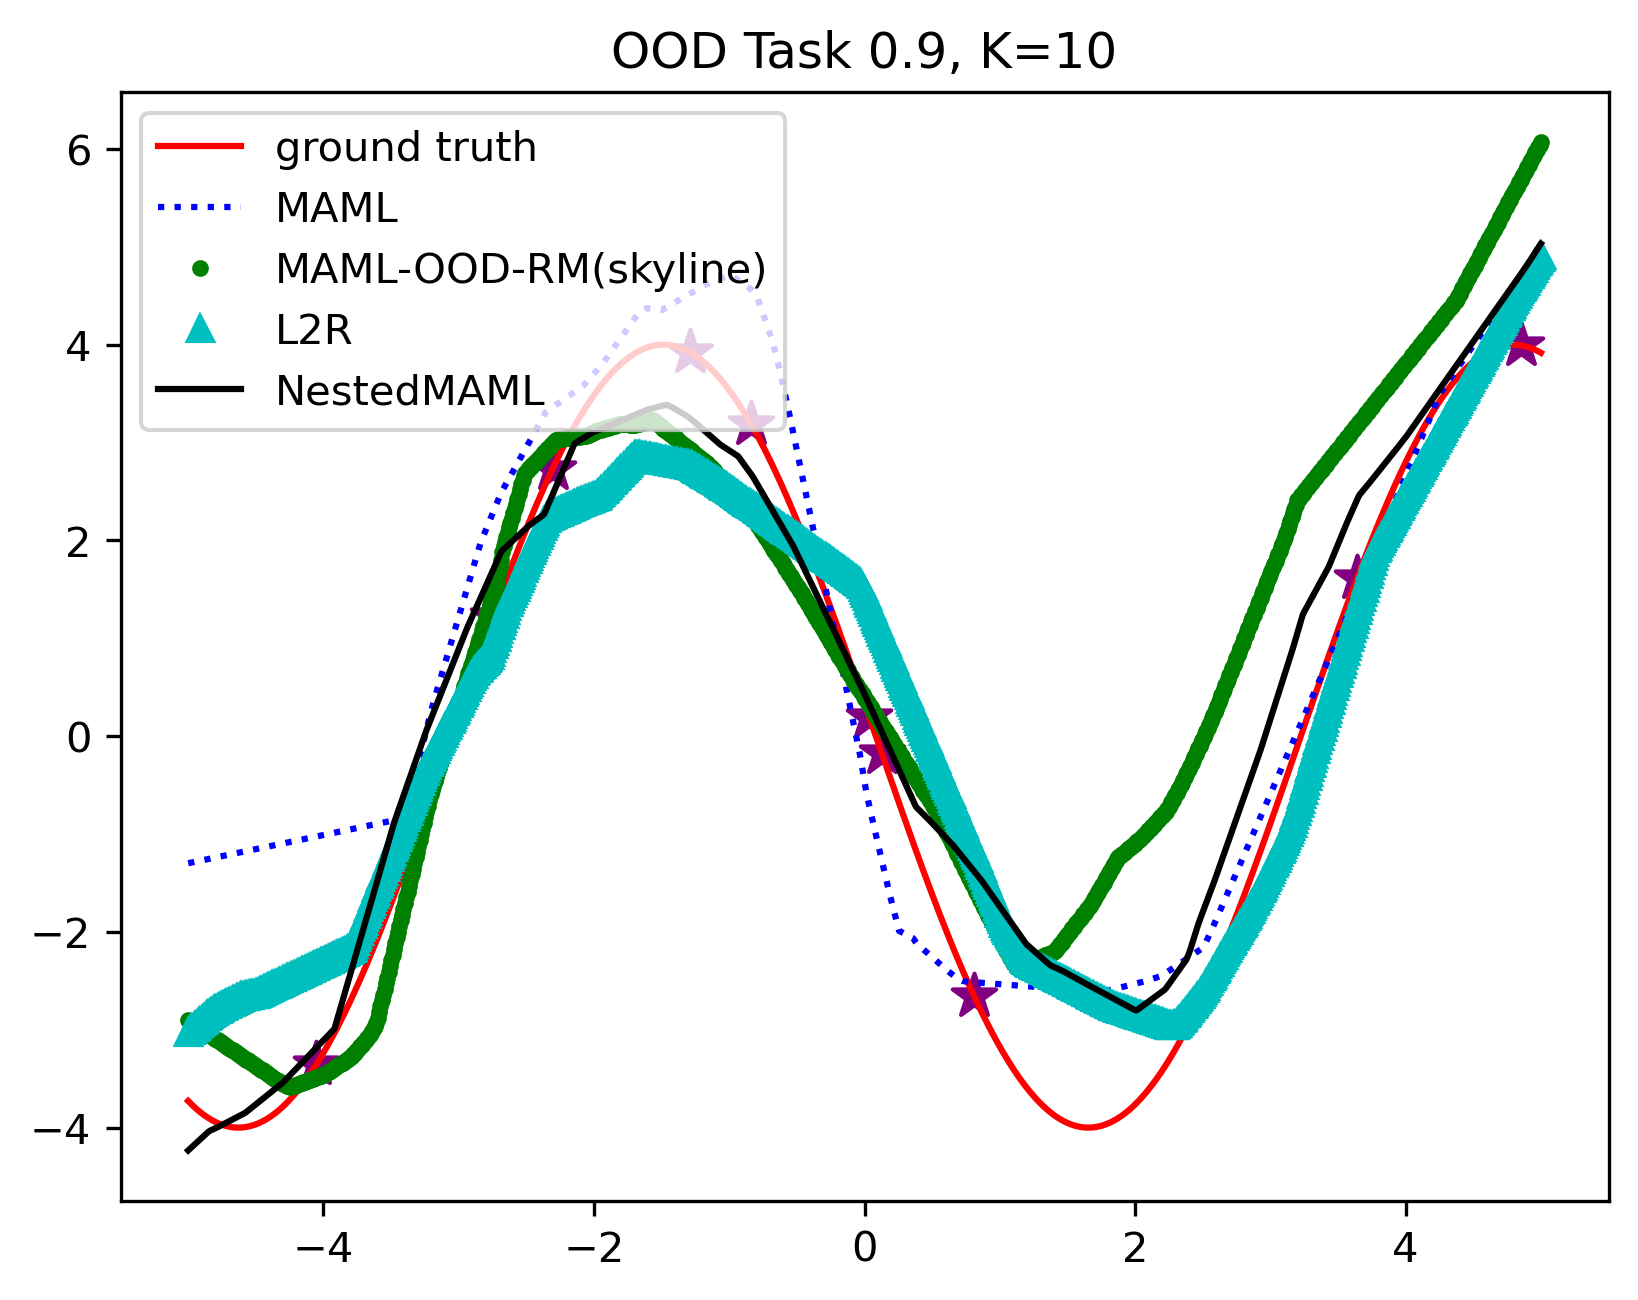
\includegraphics[width=0.9\columnwidth, height=4cm]{sine_waves/K=10_OOD_Task_0.9_Sine.png}
%         \caption{}
%     \end{subfigure}
%     \begin{subfigure}[b]{0.4\columnwidth}
%         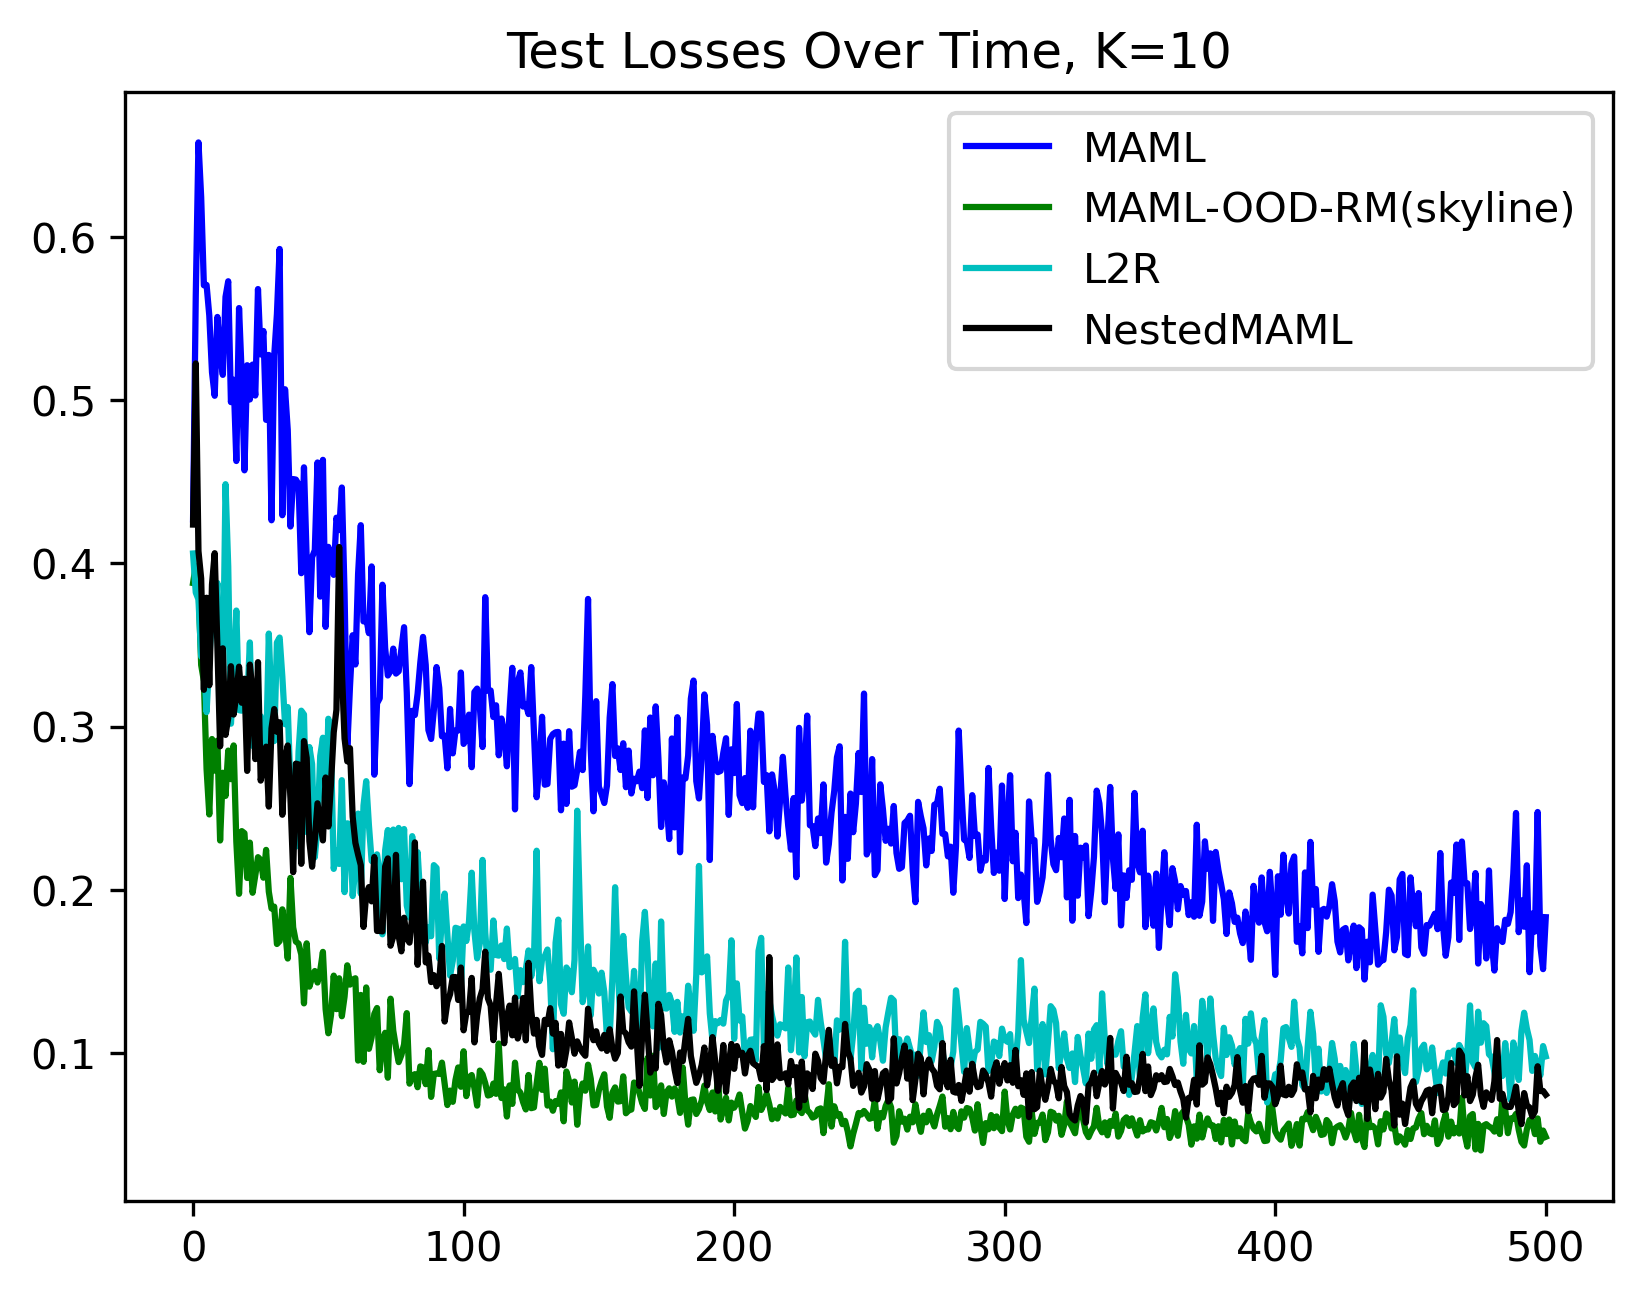
\includegraphics[width=0.9\columnwidth, height=4cm]{sine_waves/K=10_OOD_Task_0.9_ValLosses.png}
%         \caption{}
%     \end{subfigure}
%     \begin{subfigure}[b]{0.4\columnwidth}
%         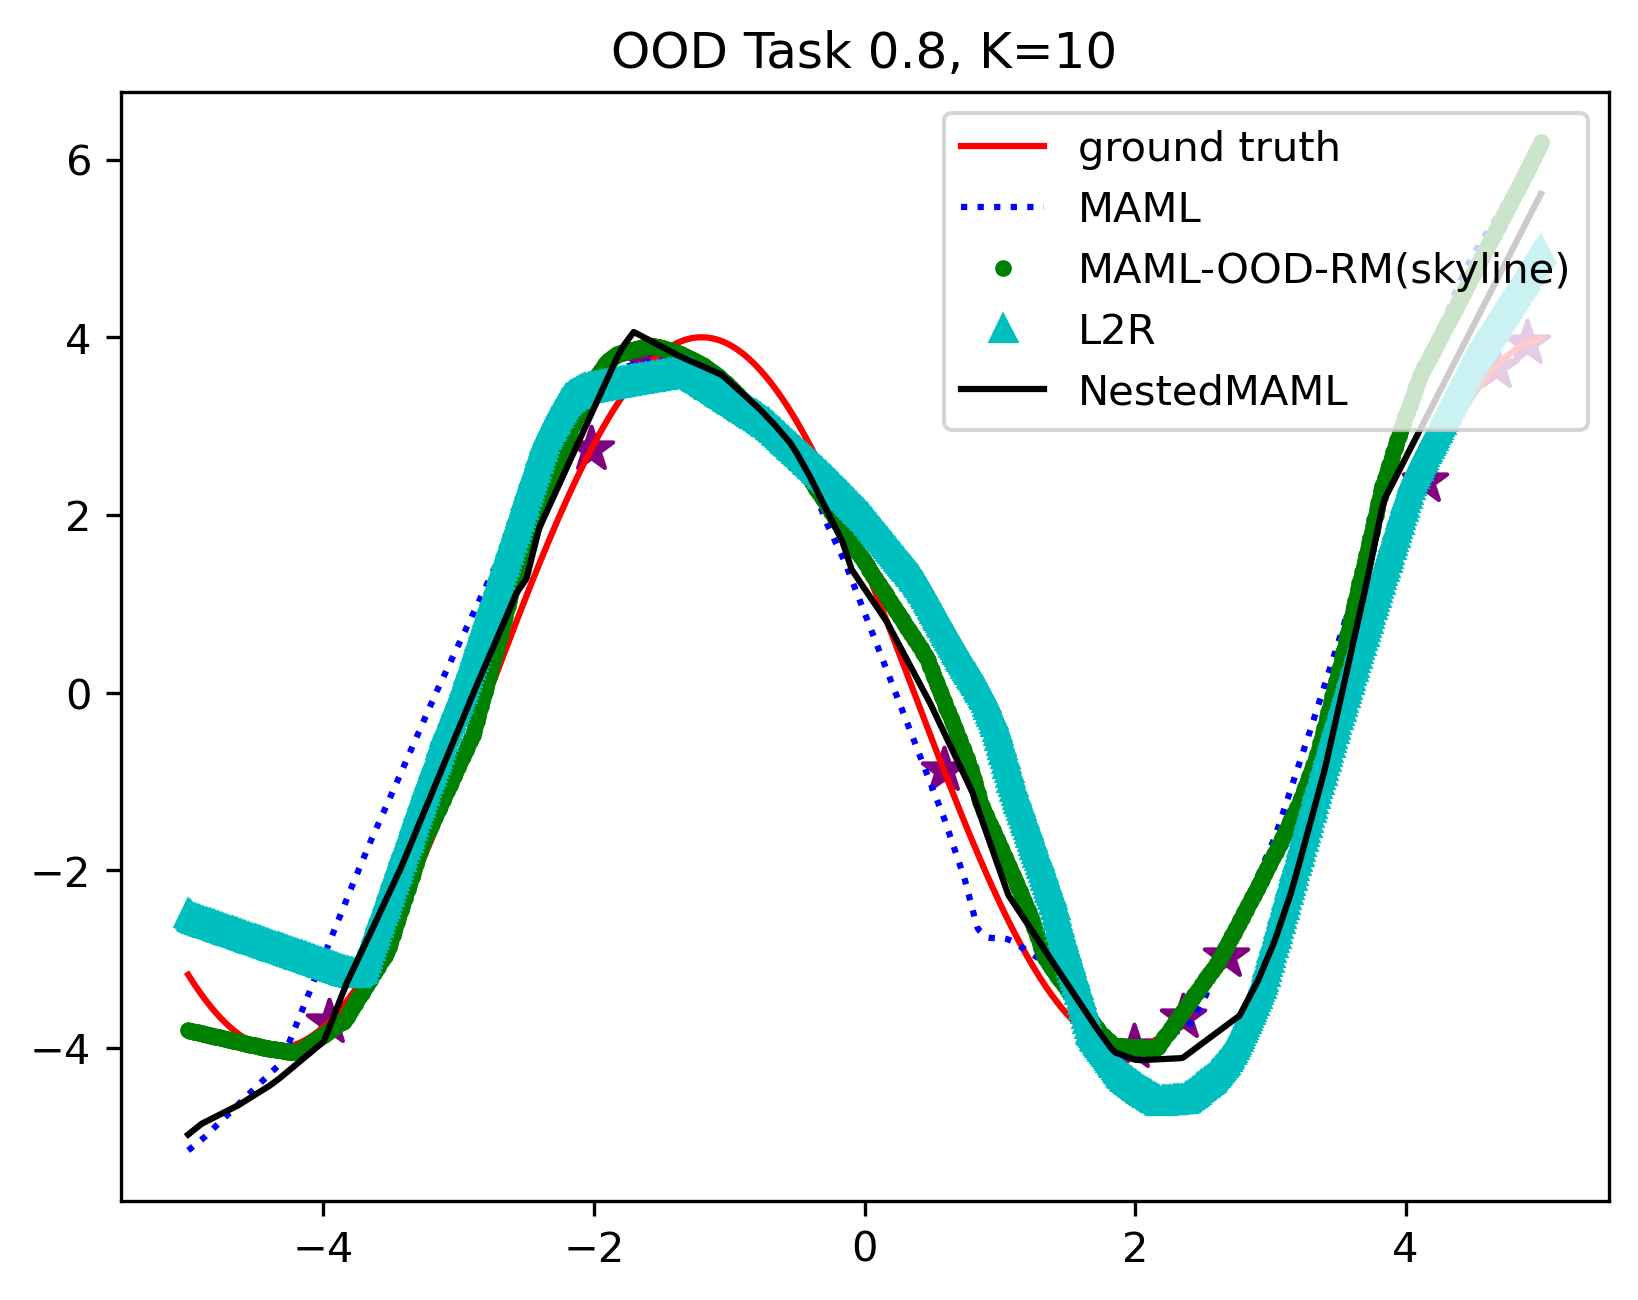
\includegraphics[width=0.9\columnwidth, height=4cm]{sine_waves/K=10_OOD_Task_0.8_Sine.png}
%         \caption{}
%     \end{subfigure}
%     \begin{subfigure}[b]{0.4\columnwidth}
%         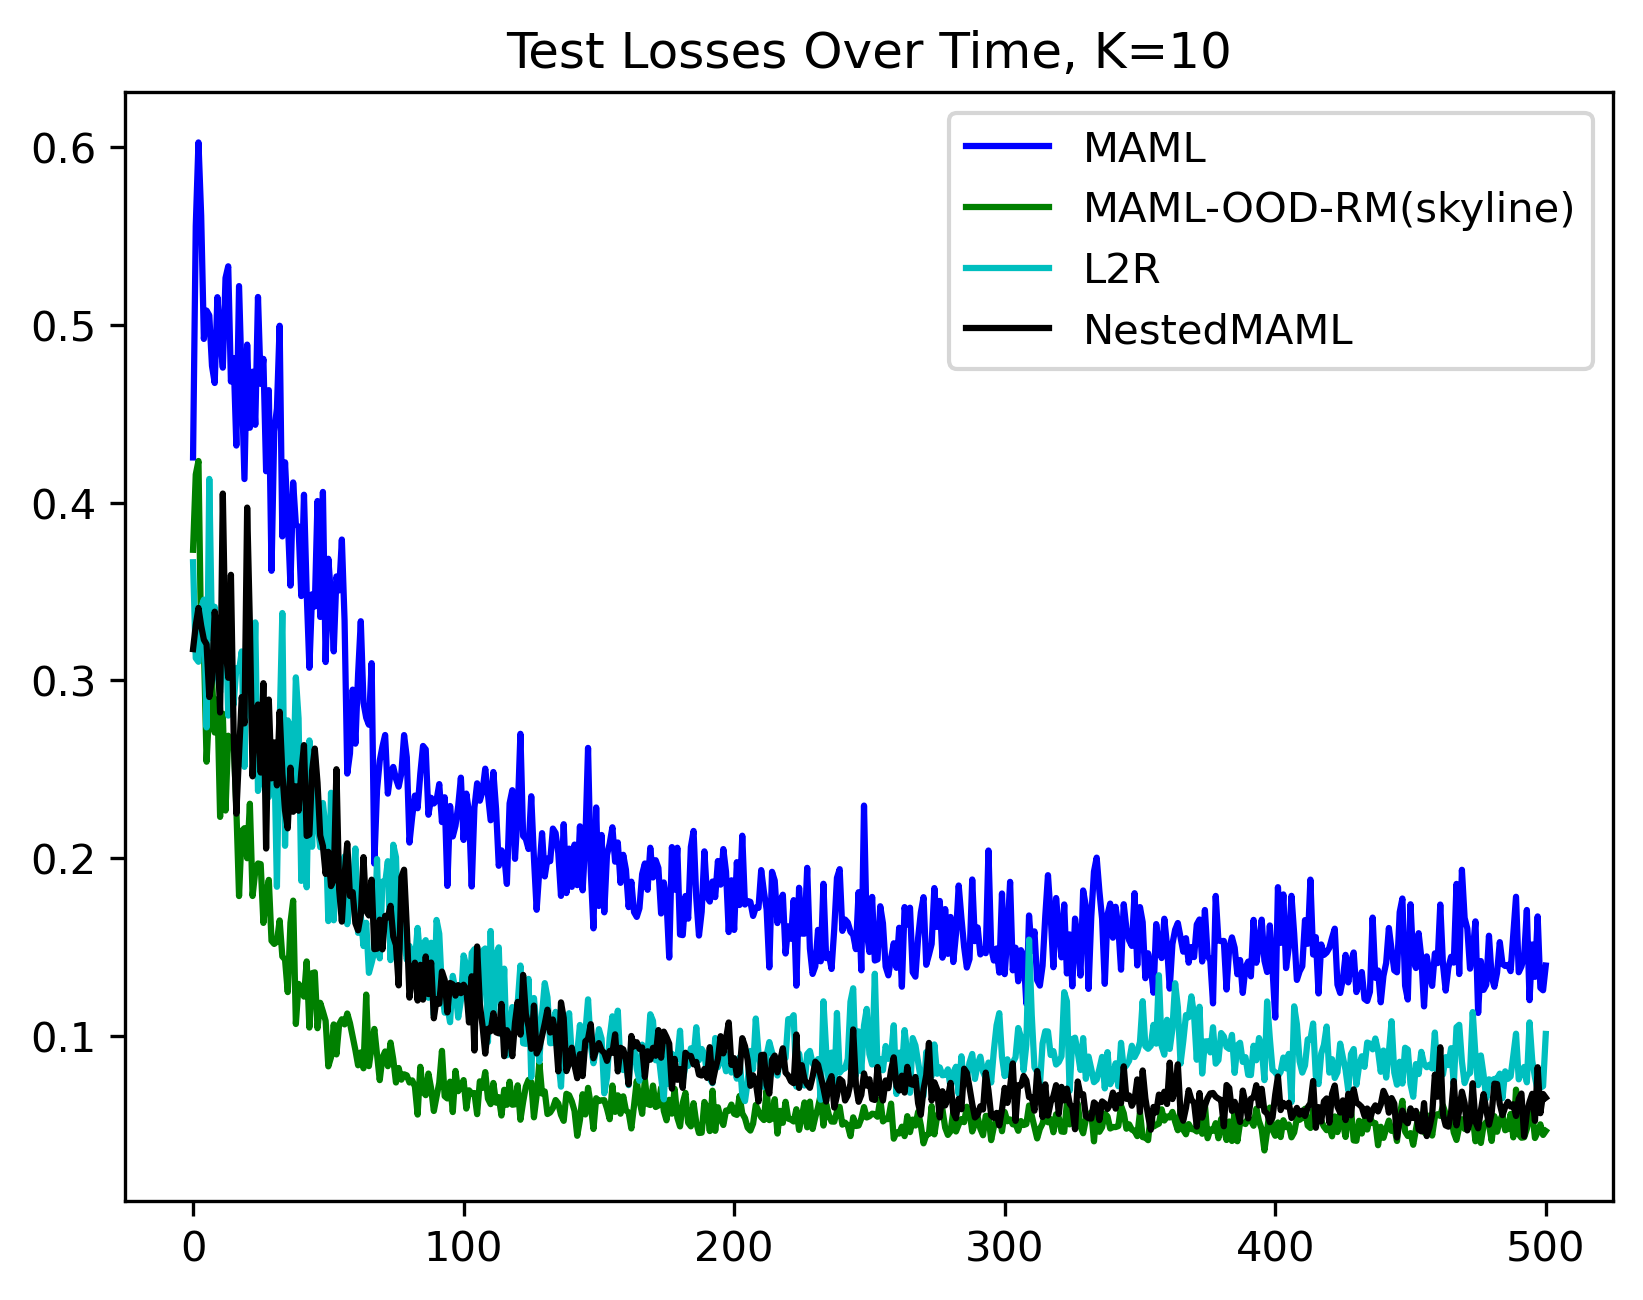
\includegraphics[width=0.9\columnwidth, height=4cm]{sine_waves/K=10_OOD_Task_0.8_ValLosses.png}
%         \caption{}
%     \end{subfigure}
%     \begin{subfigure}[b]{0.4\columnwidth}
%         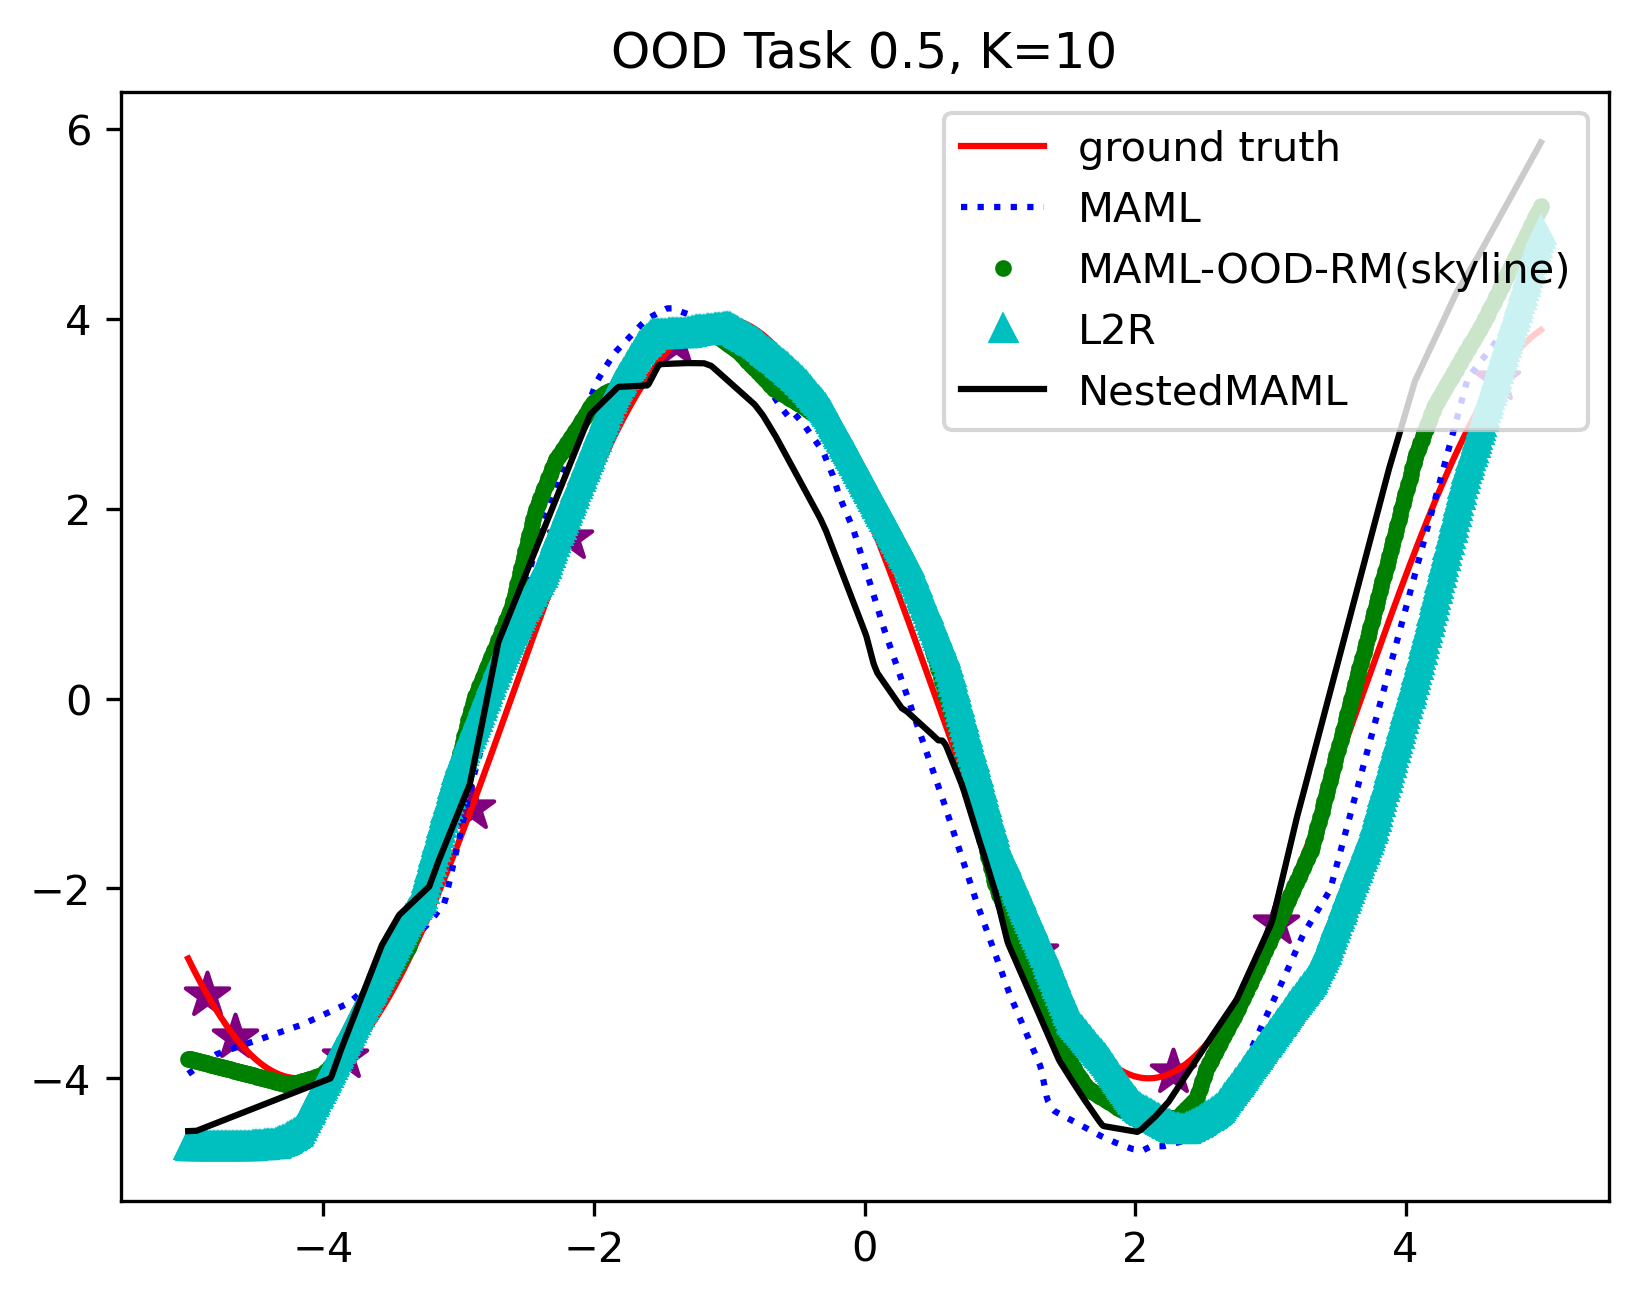
\includegraphics[width=0.9\columnwidth, height=4cm]{sine_waves/K=10_OOD_Task_0.5_Sine.png}
%         \caption{}
%     \end{subfigure}
%     \begin{subfigure}[b]{0.4\columnwidth}
%         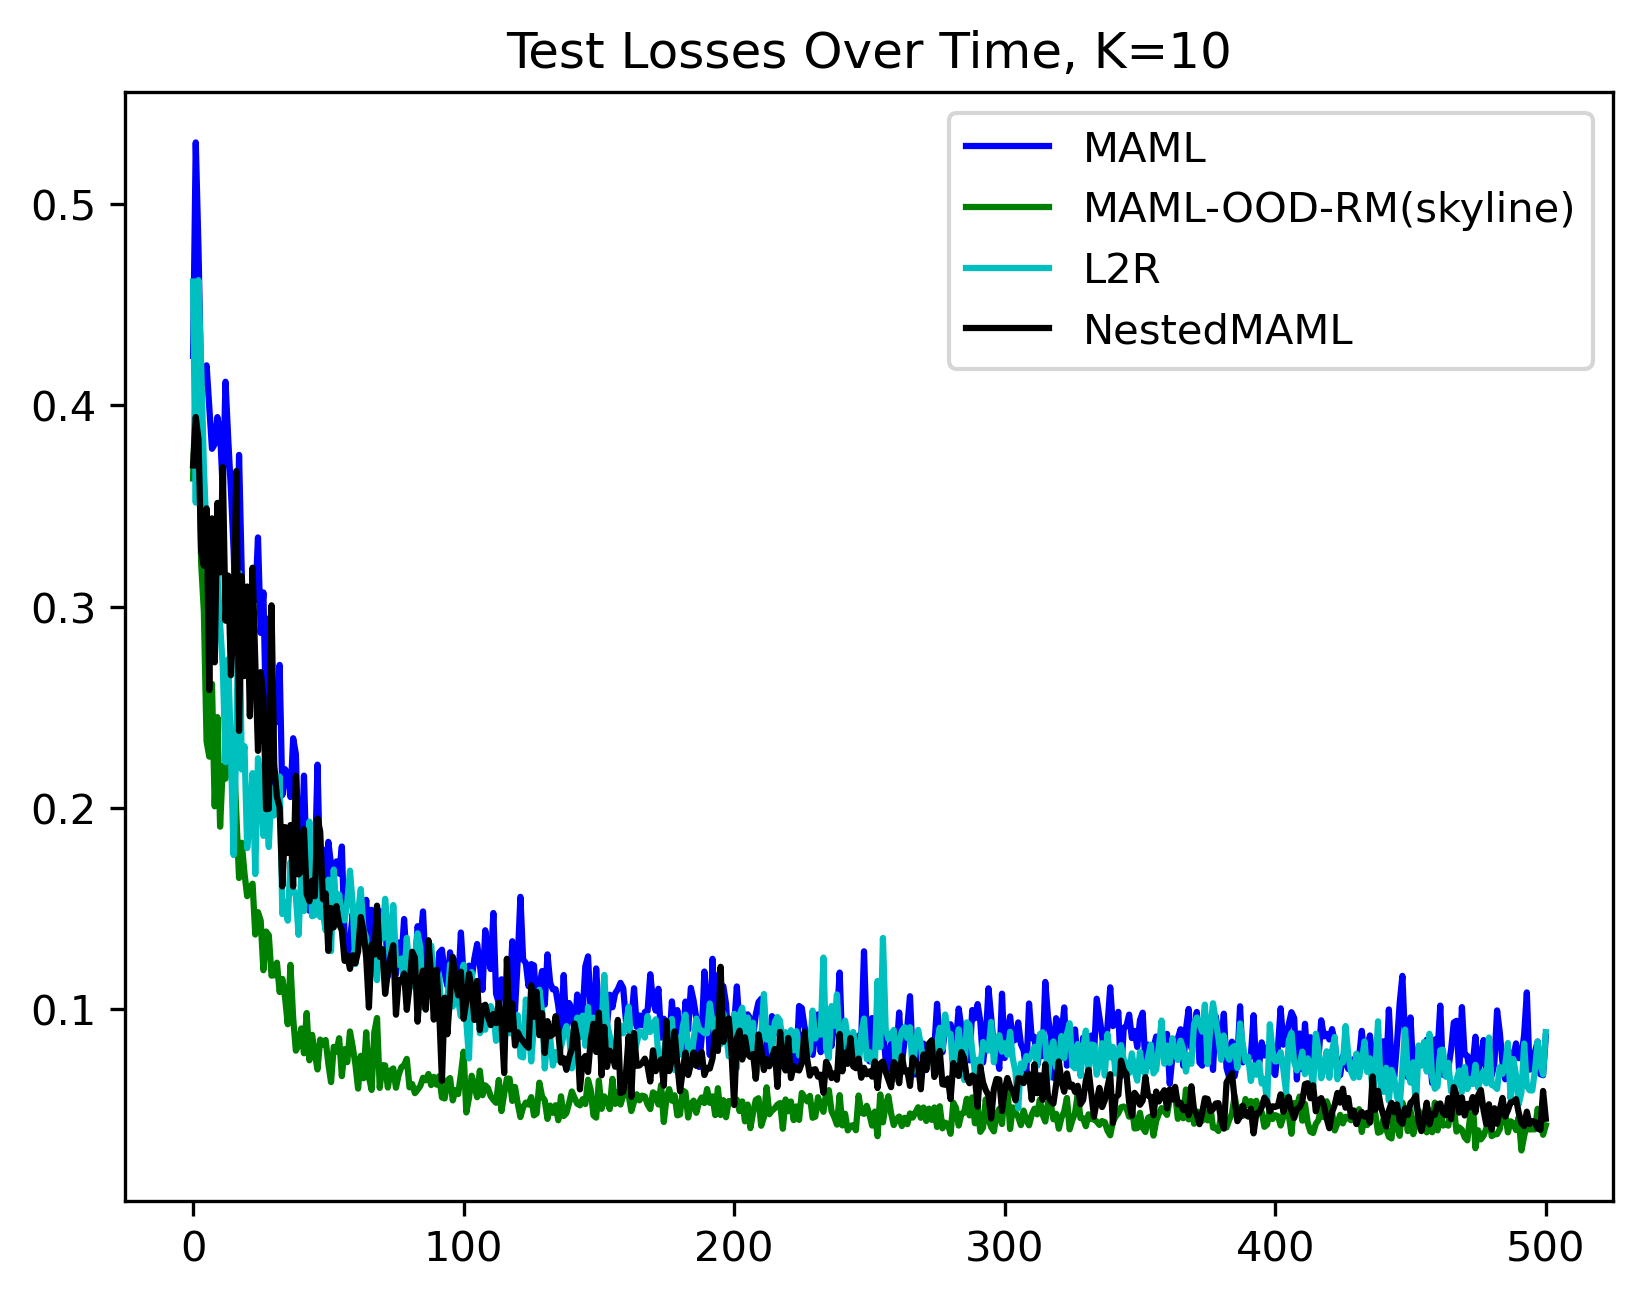
\includegraphics[width=0.9\columnwidth, height=4cm]{sine_waves/K=10_OOD_Task_0.5_ValLosses.png}
%         \caption{}
%     \end{subfigure}
%     \begin{subfigure}[b]{0.4\columnwidth}
%         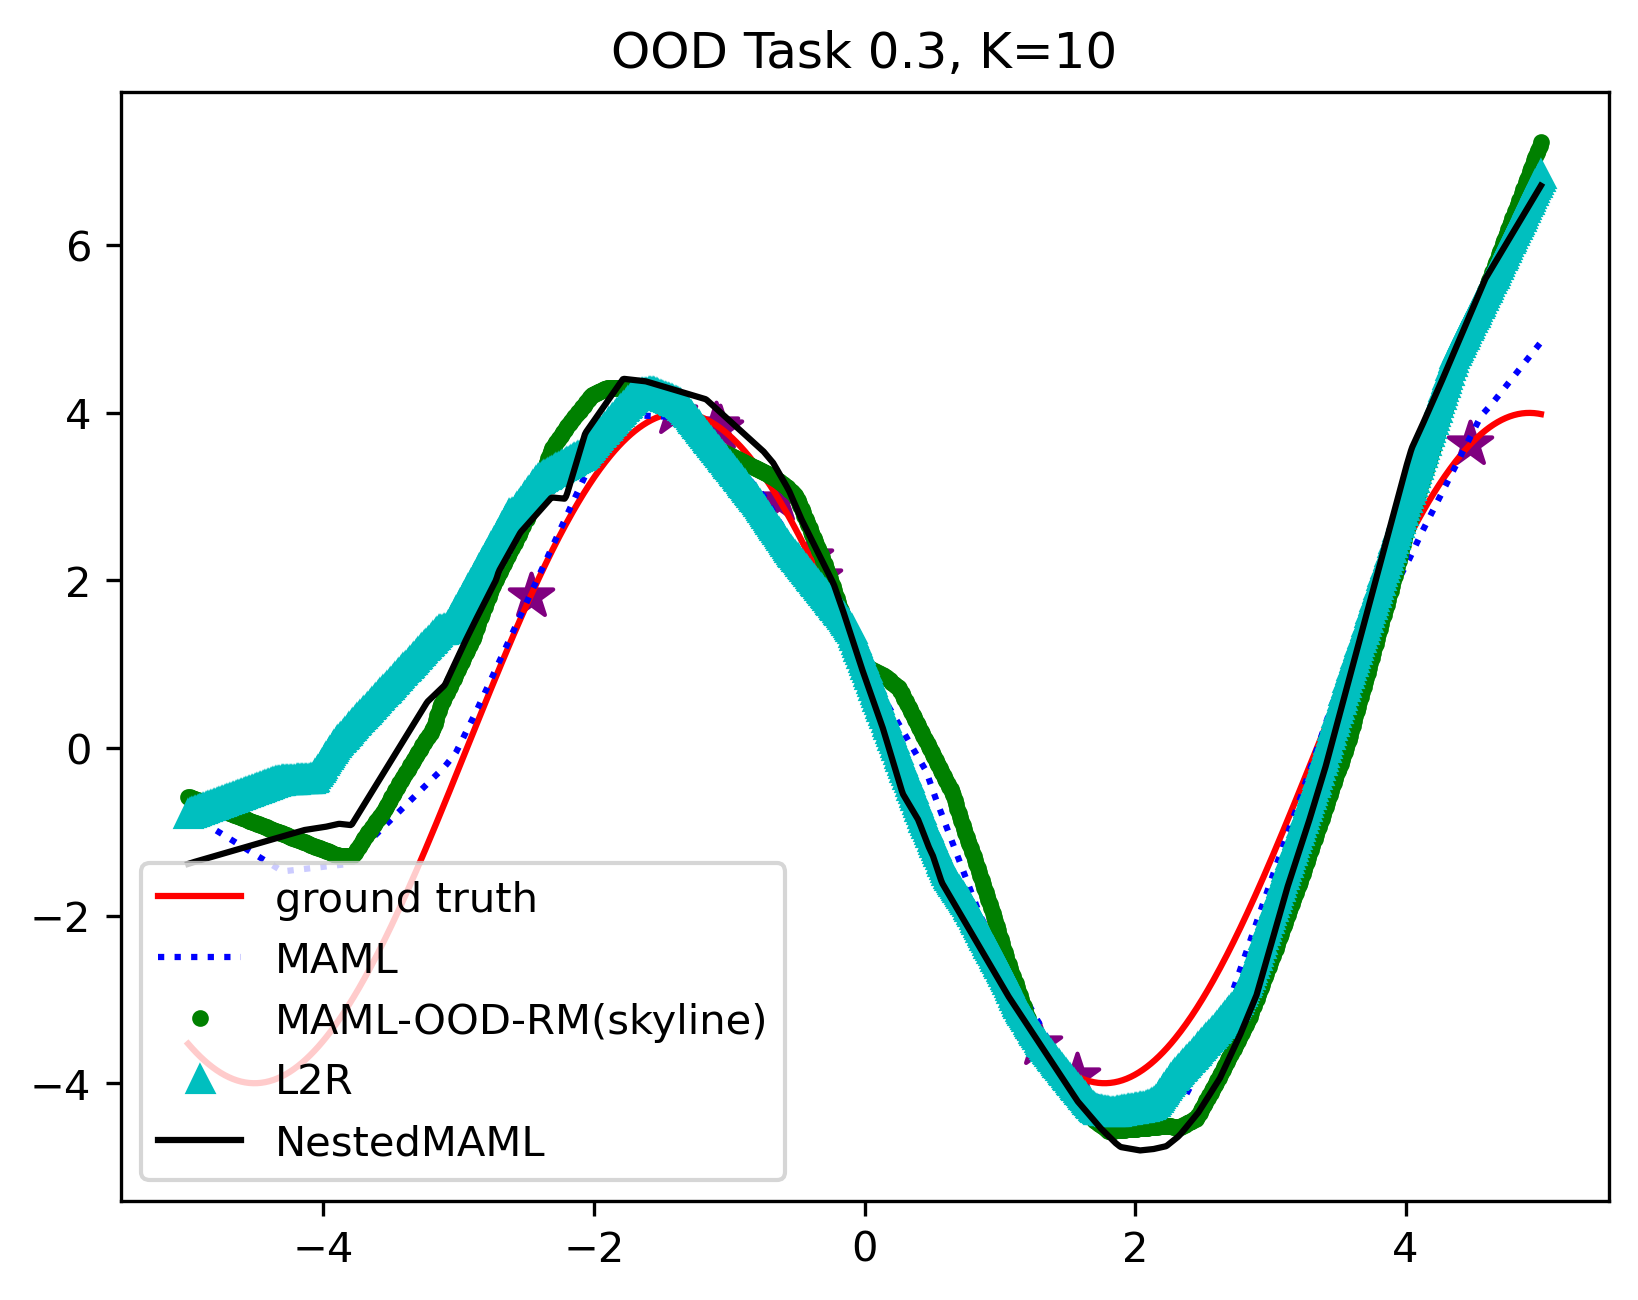
\includegraphics[width=0.9\columnwidth, height=4cm]{sine_waves/K=10_OOD_Task_0.3_Sine.png}
%         \caption{}
%     \end{subfigure}
%     \begin{subfigure}[b]{0.4\columnwidth}
%         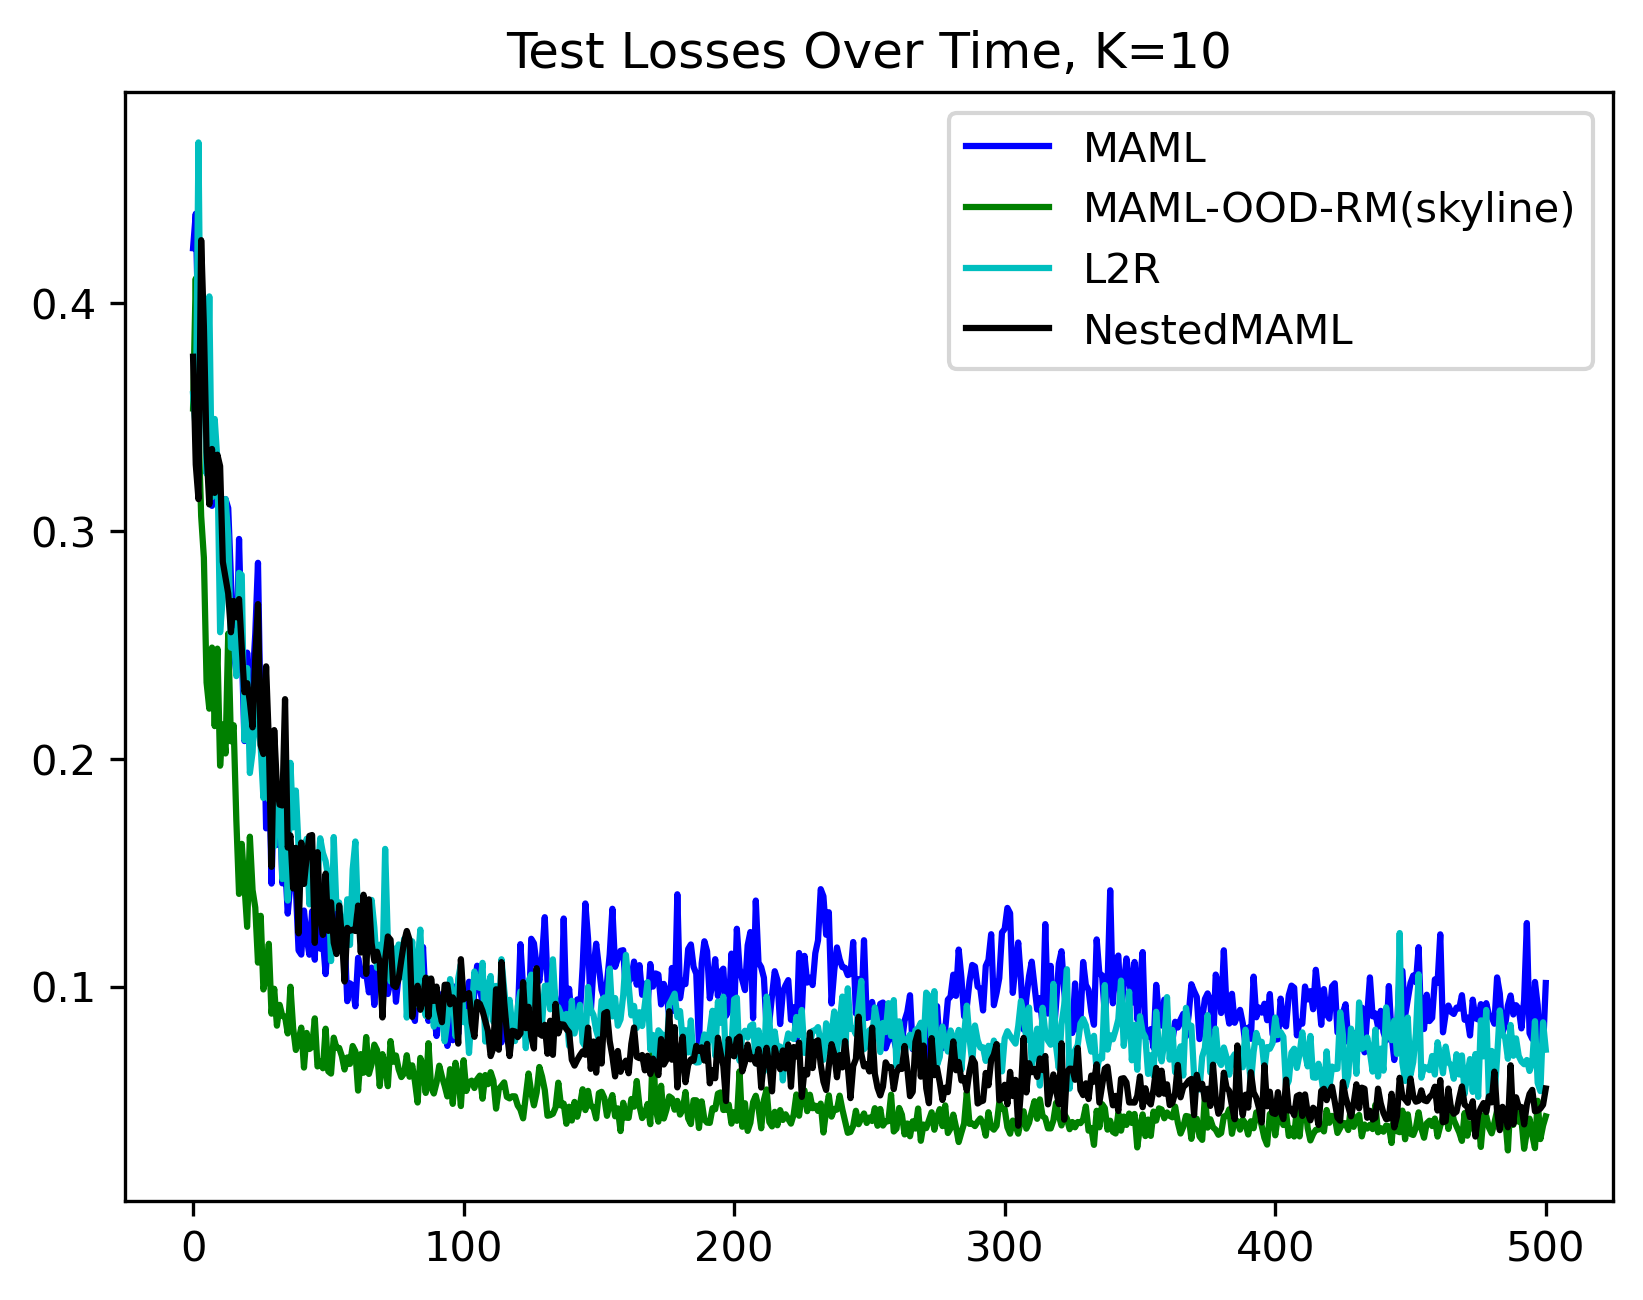
\includegraphics[width=0.9\columnwidth, height=4cm]{sine_waves/K=10_OOD_Task_0.3_ValLosses.png}
%         \caption{}
%     \end{subfigure}
%     \caption{Few-shot (K=10) adaptation for the simple regression task. Plotted by different levels of OOD Tasks (a,b) 90\%; (c,d) 80\%;. (e,f) 50\%; (g,h) 30\%;}
%     \label{synthetic_regression}
% \end{figure*}


\begin{figure*}[!htbp]
    \centering
    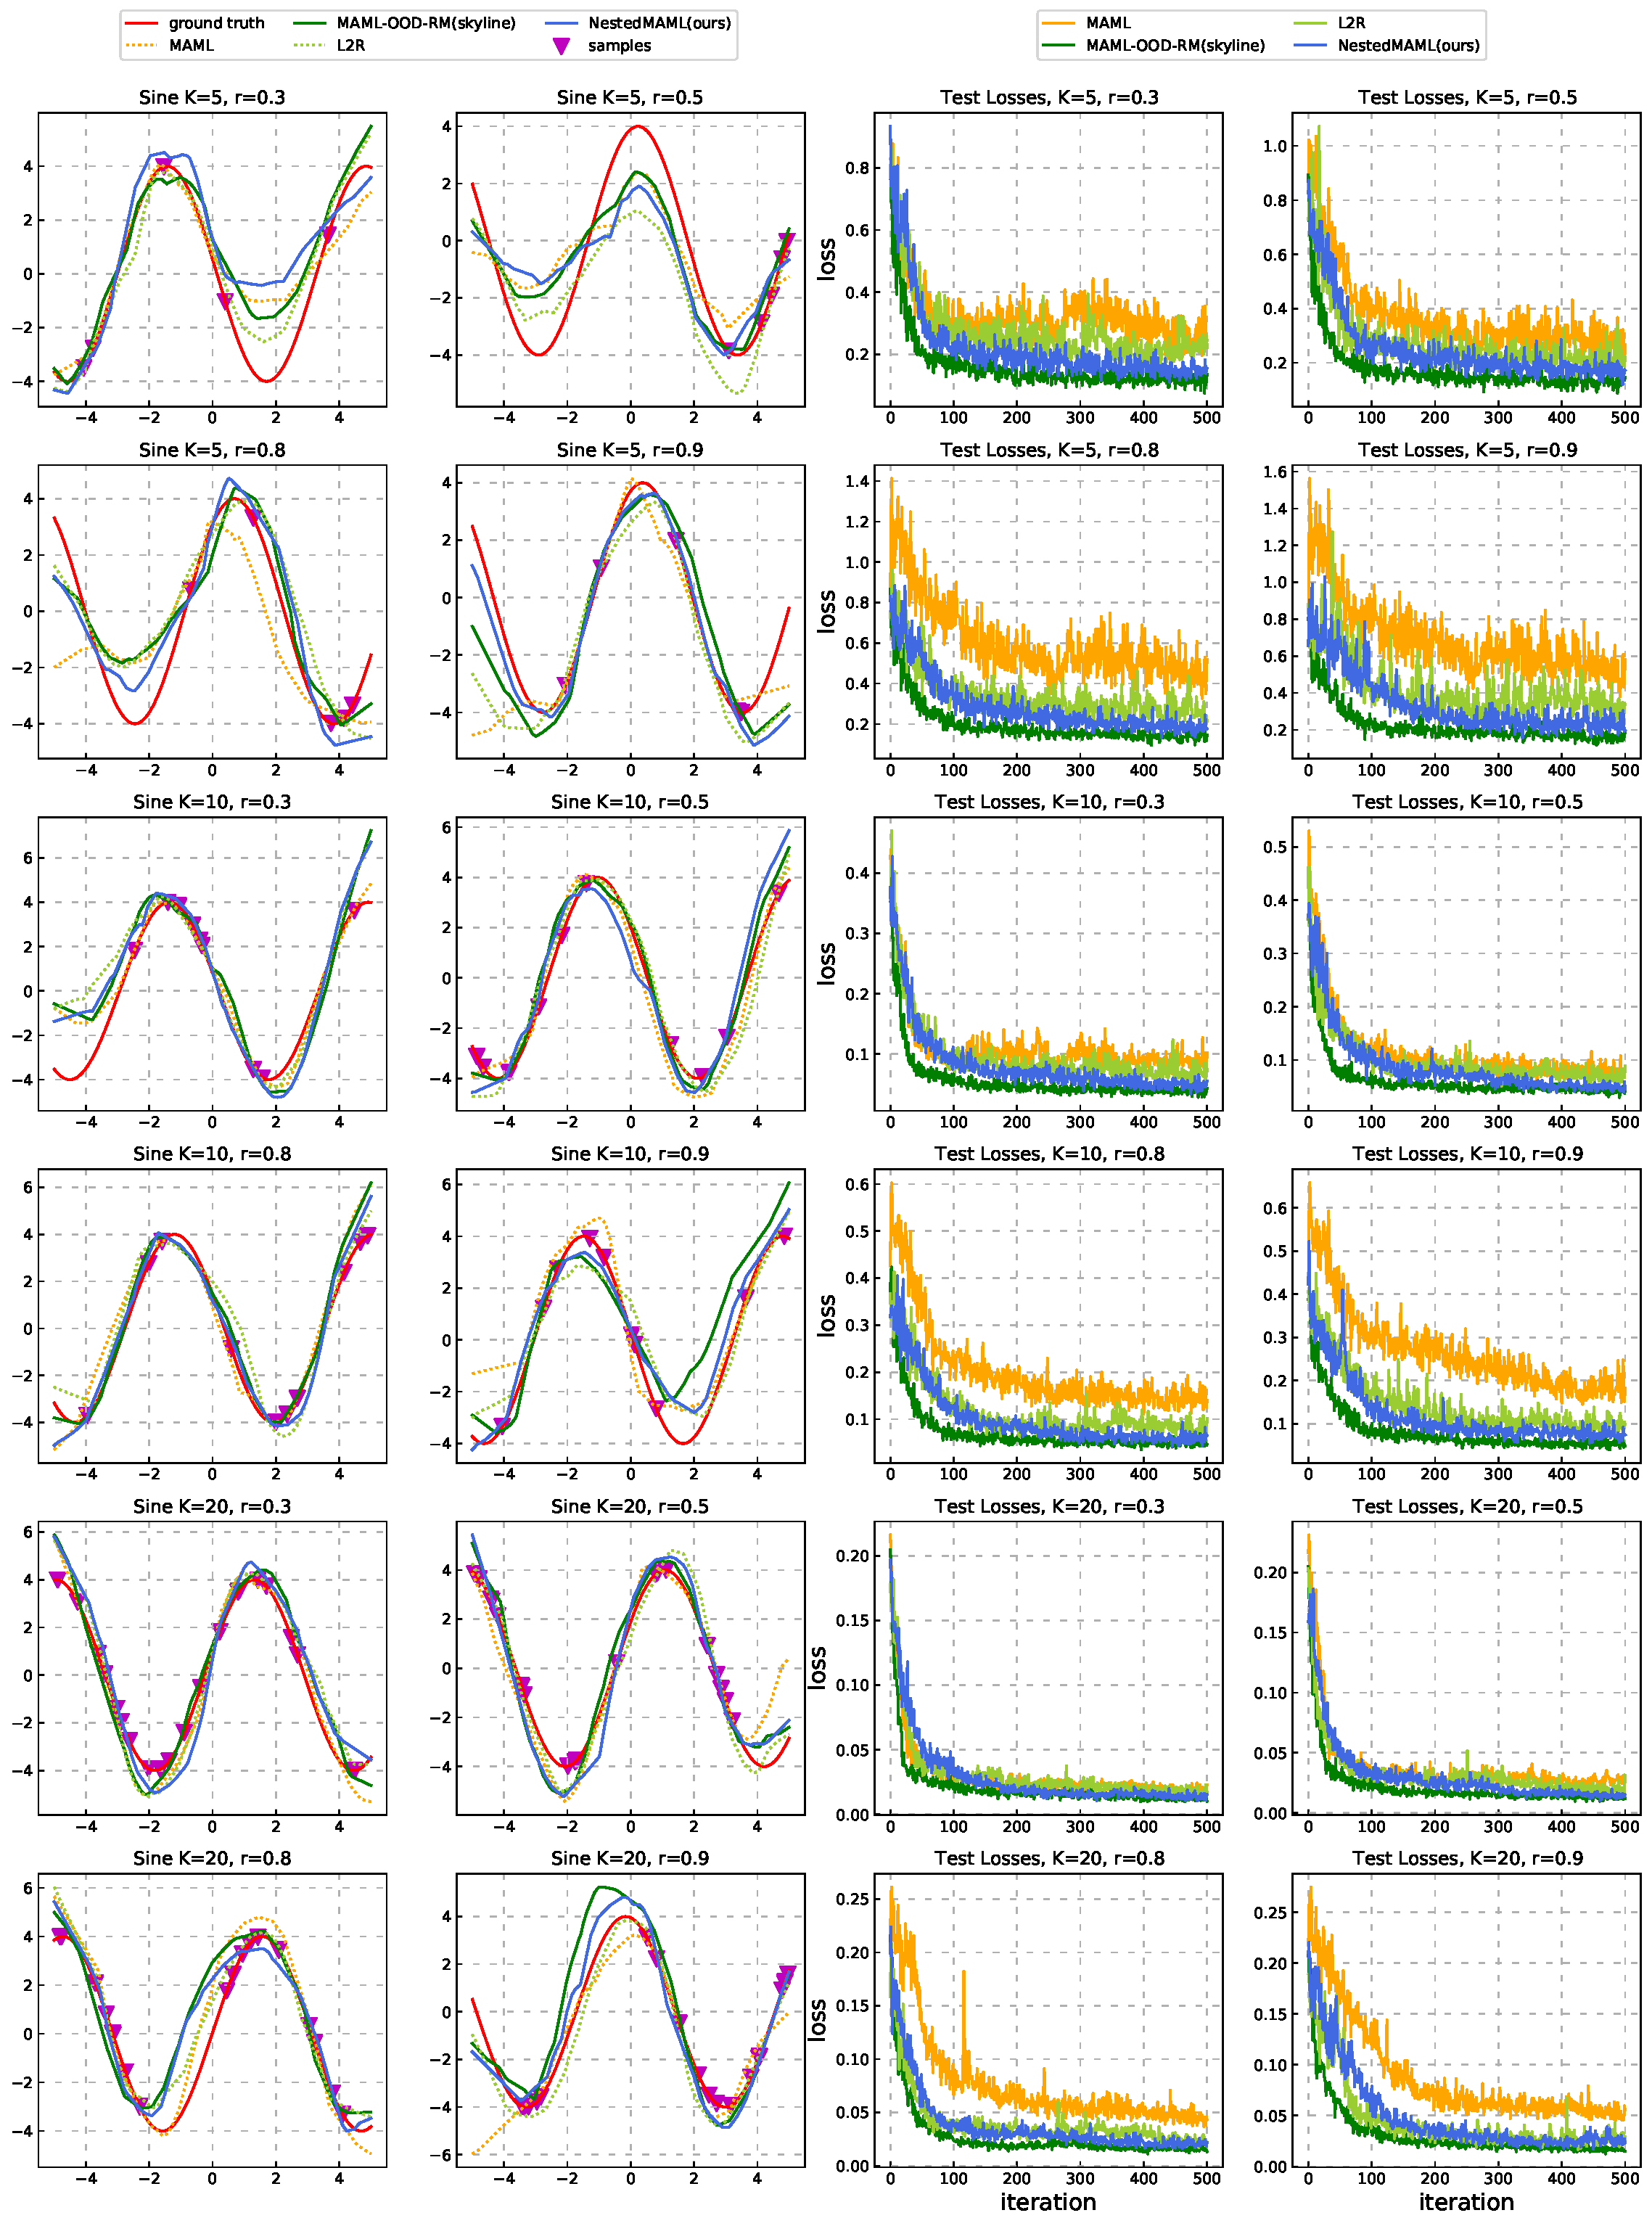
\includegraphics[width=0.96\columnwidth, height=21cm]{figs/regression.pdf}
    \caption{Results of few-shot (K=5, 10, 20) for the simple sinusoid regression task including the loss curves with respect to the number of iterations. Plotted by different levels of OOD Tasks (r = 0.3, 0.5, 0.8, 0.9).}
    \label{synthetic_regression}
\end{figure*}

\subsection{Synthetic Regression}
\textbf{Regression Setting}. To show our proposed model's robustness in the OOD task scenario, we start with a simple regression problem with outliers in the \textbf{synthetic dataset}. Specifically, during the meta-training time, each task involves $K$ samples as input and a sine wave as output, where the amplitude and phase of each sine wave are varied between tasks. More concretely, the amplitude varies within $[0.1, 5.0]$ and the phase varies within $[0, \pi]$. Datapoints from sine waves are sampled uniformly from $[-5.0, 5.0]$. In addition to in-distribution data (\textit{i.e.} data points sampled from sine waves), outliers or data points out of sine distributions (\textit{i.e.} OOD) are added into meta-training stage. To generate OOD data, we set outputs that are linear to the corresponding inputs. It is notable that, during meta-val and meta-test stages, all tasks are without any outliers. Our proposed model's intuition behind such a setting learns weights based on validation tasks and will assign higher weights to sinusoid tasks in meta-training, which could have better results. Instead, MAML uses equal weights for each meta-training task, which may not generalize good performance to unseen tasks when OOD is mixed during training. The loss function of Mean Squared Error (MSE) between prediction and the true value is applied for optimization. During meta-validation/test time, all tasks are without any outliers. Intuition: our model could learn weights based on validation tasks (sine wave) and assign higher weights to sinusoid tasks in meta-training tasks, resulting in better results. Instead, MAML uses the same weights for each task in meta-training tasks, which will not have good generalization results. 

Figure~\ref{synthetic_regression} shows the results of the \sysname{} and other baselines: \textbf{MAML}~\citep{finn2017model} and \textbf{L2R} ~\citep{ren2018learning}. The baseline \textbf{MAML-OOD-RM} corresponds to a MAML model trained just on In-Distribution (ID) tasks and will act as skyline. From Figure~\ref{synthetic_regression} and Table~\ref{tab:regres}, it is evident that \sysname{} algorithm performs better than other baseline methods and achieved low MSE error values.


\begin{table*}[!htbp]
\small
% \caption{MSE loss for the OOD experiment on various evaluation setups. \textbf{sine waves} are used as an in-distribution dataset ($\mathcal{D}_{in}$) for all experiments. }
    % \vspace{-3mm}
    \centering
% \resizebox{15cm}{3cm}{
\begin{tabular}{c|l|c|c|c|c}
    \toprule
    Shots K & Methods & r=0.3 & r=0.5 & r=0.8 & r=0.9   \\
    \midrule
    \multirow{4}{*}{5} & MAML-OOD-RM(skyline)  & 0.1357 & 0.1460 & 0.1457 & 0.1830 \\
    \cline{2-6} 
    & MAML  & 0.2448  & 0.2658 & 0.5200 & 0.5807 \\
    & L2R   & 0.2228  & 0.2225 & 0.2137 & 0.3361 \\
    & \sysname{} (ours)  & \textbf{0.1548} & \textbf{0.1725} & \textbf{0.1761} & \textbf{0.1971} \\
    \midrule
    \multirow{4}{*}{10} & MAML-OOD-RM(skyline)  & 0.0430 & 0.0425 & 0.0466 & 0.0485 \\
    \cline{2-6} 
    & MAML  & 0.1015 & 0.0865 & 0.1397 &  0.1831 \\
    & L2R   & 0.0723 & 0.0888 & 0.1022 &  0.0978 \\
    & \sysname{} (ours)  & \textbf{0.0552} & \textbf{0.0458} & \textbf{0.0653} & \textbf{0.0743} \\
    \midrule
    \multirow{4}{*}{20} & MAML-OOD-RM(skyline)  & 0.0102 & 0.0120  & 0.0131 & 0.0150 \\
    \cline{2-6} 
    & MAML  & 0.0228 &  0.0278  & 0.0432 & 0.0553 \\
    & L2R   & 0.0169 &  0.0314  & 0.0219 & 0.0289 \\
    & \sysname{} (ours)  &  \textbf{0.0152} & \textbf{0.0153} & \textbf{0.0221} & \textbf{0.0231} \\
    \bottomrule
\end{tabular}
\caption{MSE loss for the OOD experiment on various evaluation setups. \textbf{sinusoid} is used as an in-distribution dataset ($\mathcal{D}_{in}$) for all experiments. }
\label{tab:regres}

\end{table*}

\subsection{More Experimental Details} \label{app:exp_details}

\paragraph{Datasets: }\textbf{\textit{Mini}-ImageNet}~\citep{ravi2016optimization} contains 60,000 images of size $84\times84\times3$ from 100 classes. We use the split proposed in~\cite{ravi2016optimization}: 64 classes for training, 12 classes for validation and 24 classes for testing. \textbf{SVHN}~\citep{netzer2011reading}, a street view house numbers dataset, contains 26,032 images of  size $32\times32\times3$ from 10 digits classes. \textbf{FashionMNIST}~\citep{xiao2017fashion}, a fashion dataset(\textit{i.e.} clothes, shoes, \textit{etc}), contains 60,000 grayscale images of size $28\times28$ pixels from 10 classes.


% \textbf{Datasets:} \textbf{mini-ImageNet}~\citep{ravi2016optimization} consists of 60,000 color images scaled down to $84\times84$ divided into 100 classes with 600 examples each. We use the split proposed in~\cite{ravi2016optimization}, which consists of 64 classes for training, 12 classes for validation and 24 classes for testing. This dataset is considered as in-distribution data ($\mathcal{D}_{in}$) for the experimental setting.
% \textbf{SVHN}~\citep{netzer2011reading} is a street view house numbers dataset. It consists of 26,032 color images of $32\times32$ pixels, from 10 digits classes.
% \textbf{FashionMNIST}~\citep{xiao2017fashion} consists of 60,000 grayscale images of $28\times28$ pixels, from 10 classes from various fashion styles (\textit{i.e.} clothes, shoes, \textit{etc}). Both SVHN and FashionMNIST datasets are used as out-of-distribution outliers ($\mathcal{D}_{out}$) for mini-ImageNet. 

\paragraph{Details of Settings: } As aforementioned, our backbone follows the same architecture as the embedding function used by \citep{finn2017model}. Specially, the backbone structure consists of 4 modules, each of which contains a $3\times3$ convolutions and 64 filters, followed by batch normalization, a ReLU, and a $2\times2$ max-pooling with stride 2. To reduce overfitting, 32 filters per layer are considered. We use the same model for OOD and ID tasks during the meta-training stage, so it's necessary to make sure the image sizes are consistent. We resize the image size of SVHN and FashionMNIST to $84\times84\times3$ which is consistent with \textit{mini}-ImageNet when evaluating the task-level weighting scheme. We also use the same backbone when evaluating the instance-level weighting scheme. Cross entropy loss function is used for these two schemes. 


% \paragraph{Parameter Tuning for Task-level Scheme in Sec.\ref{sec:exp_task-level}: }
\paragraph{Parameter Tuning for Task-level Scheme: }All baseline approaches follow the original implementation including hyper-parameters. For our \sysname{} algorithm, all step sizes ($\alpha, \eta, \gamma$) are chosen from $\{0.0001, 0.001, 0.01, 0.1\}$. Batch size ($m,n$) are chose from $\{4, 10, 20, 25, 32\}$. The number of iterations are chosen from $\{10,000,\enspace 20,000,\enspace 30,000,\enspace 40,000,\enspace 60,000\}$. The number of clusters used in K-means is chosen from $\{50,\enspace 200,\enspace 1,000,\enspace 5,000,\enspace 10,000\}$. The selected best ones are: Fast model parameters step size $\alpha=0.01$, meta parameters step size $\eta=0.001$, weight update step size $\gamma=0.1$; mini-batch size $m=n=10$; the number of iterations in $30\%,60\%$ are $30,000$, $90\%$ is $60,000$ respectively. The number of clusters is 200. 

% \subsection{Instance-level weighting scheme with noisy labels}
% \paragraph{Parameter Tuning for Instance-level Scheme in Sec.\ref{sec:exp_instance-level}: } 
\paragraph{Parameter Tuning for Instance-level Scheme: }Tuning hyper-parameters follows the same aforementioned strategy. The selected best ones are: Fast model parameters step size $\alpha=0.01$, meta parameters step size $\eta=0.001$, weight update step size $\gamma=0.01$; mini-batch size $m=n=10$; the number of iterations in $20\%,30\%,50\%$ are $20,000$. The number of clusters is 200.  

Other related hyperparameters are kept the same with MAML. For example, 5 gradient steps are used when training the backbone in these two schemes, and 10 gradient steps during the meta-test stage. The number of instances in the query set of each task is 15.
